% =====================================================================
%  Mecánica I · Tema 3
%  El problema de dos cuerpos. Colisiones
%  Compilar:  latexmk -lualatex tema3.tex
% =====================================================================
\documentclass[11pt,a4paper,twoside]{article}
\usepackage{estilo-oscuro}

\renewcommand{\cabeceraimpar}{Tema 3 · Dos cuerpos y colisiones}
\renewcommand{\cabecerapar}{Mecánica I}

\hypersetup{pdftitle={Tema 3. El problema de dos cuerpos. Colisiones},
  pdfauthor={Daniel Martín Guerrero},pdfsubject={Mecánica I}}

% ----- notación propia del tema ---------------------------------------
\usetikzlibrary{decorations.pathreplacing,babel}
\newcommand{\ext}{^{(\mathrm{ext})}}
\newcommand{\inn}{^{(\mathrm{int})}}
\newcommand{\cm}{_{\mathrm{CM}}}
\newcommand{\Rcm}{\vb{R}\cm}
\newcommand{\Vcm}{\vb{V}\cm}
\newcommand{\vrel}{\vb{v}_{12}}
\newcommand{\lab}{\textup{\textsc{lab}}}
\newcommand{\scm}{\textup{\textsc{cm}}}

\begin{document}

% =====================================================================
%  PORTADA
% =====================================================================
\begin{titlepage}
\newgeometry{left=27mm,right=27mm,top=20mm,bottom=20mm}
\pagecolor{fondo}\color{texto}
\centering

\includegraphics[width=0.30\textwidth]{figs/logo_usal.png}\par
\vspace{6mm}
{\color{tenue!60}\rule{\textwidth}{0.4pt}}\par
\vspace{4mm}
{\small\color{tenue}\textls[180]{\textsc{Facultad de Ciencias}}\quad·\quad
 \textls[180]{\textsc{Grado en Física}}}\par
\vspace{13mm}
{\color{cian}\textls[220]{\textsc{Mecánica I}}}\par
\vspace{2.2mm}
{\small\color{tenue}\textls[200]{\textsc{Tema 3}}}\par
\vspace{9mm}
{\fontsize{29}{31}\selectfont\bfseries El problema de dos cuerpos.\\[1.5mm] Colisiones\par}
\vspace{7mm}
{\color{tenue}\rule{0.22\textwidth}{0.4pt}}\par
\vspace{5mm}
{\itshape Masa reducida · Percusión y coeficiente de restitución\\
Sistemas {\upshape\lab{}} y {\upshape\scm{}} · Diagrama de Landau · Choques oblicuos y rebotes\par}
\vfill
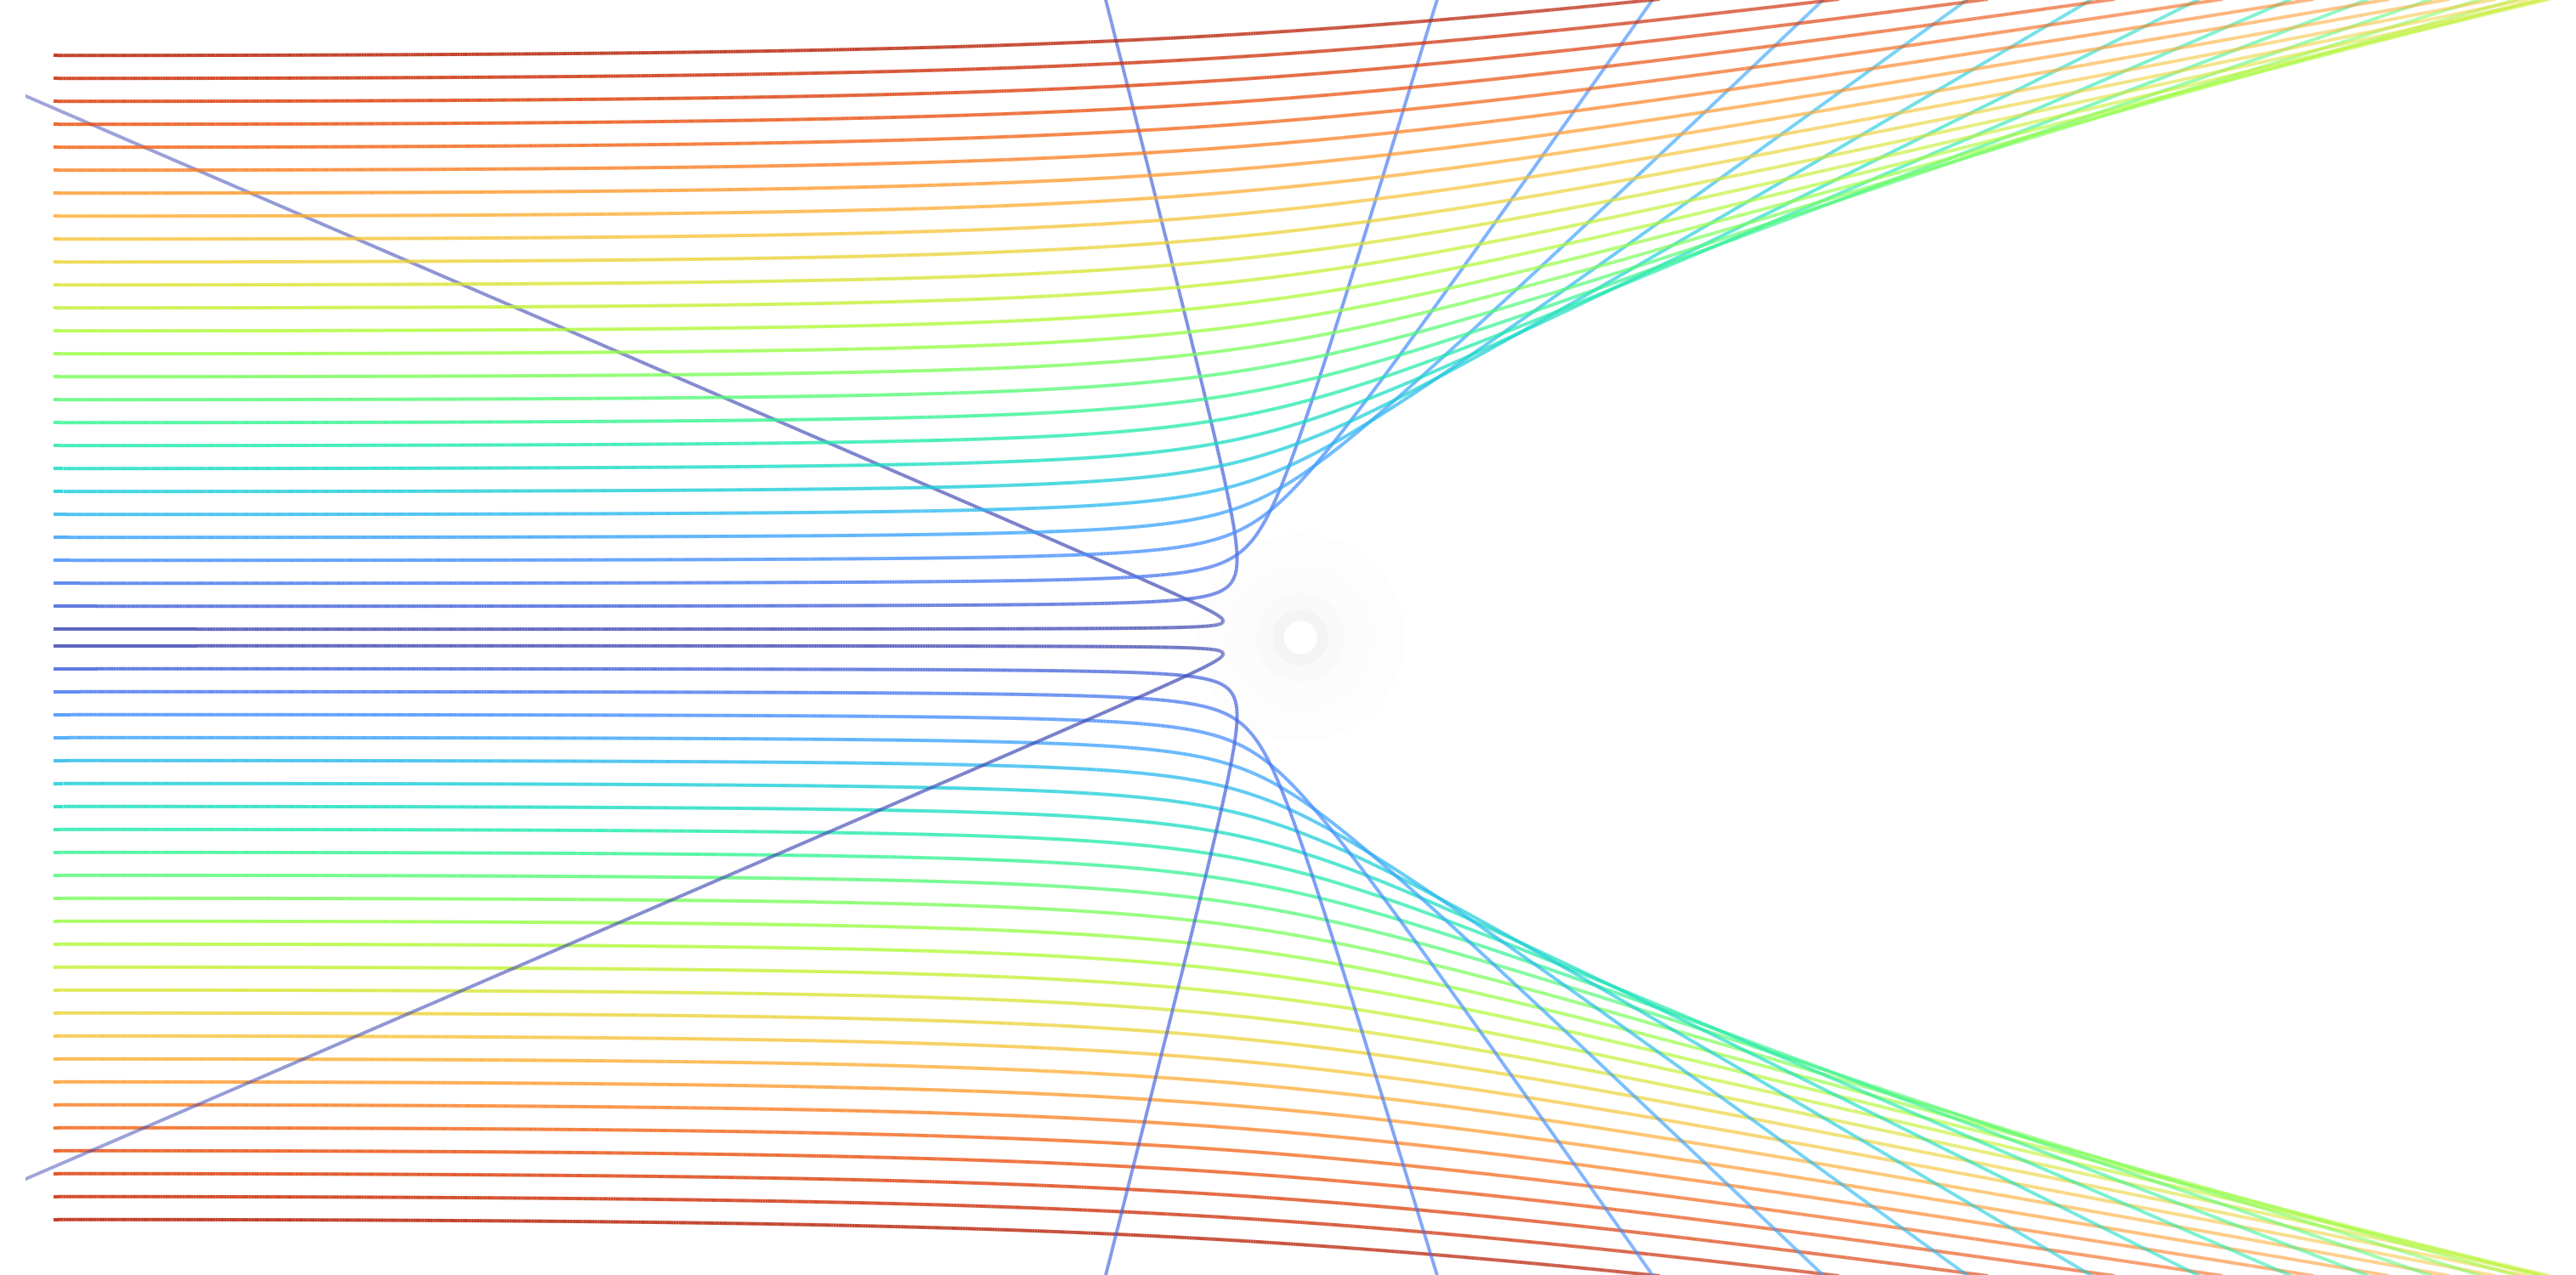
\includegraphics[width=1.0\textwidth]{figs/portada.png}\par
\vfill
{\small
$\displaystyle \mu=\frac{m_{1}m_{2}}{m_{1}+m_{2}},\qquad
v_{1}'-v_{2}'=-e\,(v_{1}-v_{2}),\qquad
\tan\alpha=\frac{\sin\theta}{m_{1}/m_{2}+\cos\theta}$\par}
\vspace{9mm}
{\color{tenue!60}\rule{\textwidth}{0.4pt}}\par
\vspace{3mm}
{\small
\begin{tabular*}{\textwidth}{@{}l@{\extracolsep{\fill}}c@{\extracolsep{\fill}}r@{}}
{\color{cian}\scriptsize\textls[200]{\textsc{Autor}}} &
{\color{cian}\scriptsize\textls[200]{\textsc{Asignatura}}} &
{\color{cian}\scriptsize\textls[200]{\textsc{Apuntes formalizados}}}\\[0.6mm]
Daniel Martín Guerrero & Mecánica I (100810) & {\color{tenue}Salamanca, curso 2026/2027}\\
 & {\color{tenue}Teoría y seminario de problemas} & \\
\end{tabular*}}
\restoregeometry
\end{titlepage}

% =====================================================================
\setcounter{page}{2}
\tableofcontents
\clearpage

% =====================================================================
\section{El problema de dos cuerpos}
\label{sec:dos-cuerpos}
% =====================================================================

Es el sistema de partículas más sencillo y el único que, en general, se resuelve
reduciéndolo a problemas de \emph{una} partícula. Notación: $M=m_{1}+m_{2}$,
\[
  \vb{r}\defeq\vb{r}_{12}=\vb{r}_{1}-\vb{r}_{2},\qquad
  \vrel\defeq\dot{\vb{r}}=\vb{v}_{1}-\vb{v}_{2},\qquad
  \Rcm=\frac{m_{1}\vb{r}_{1}+m_{2}\vb{r}_{2}}{M},\qquad \Vcm=\dot{\vb{R}}\cm .
\]

\begin{definicion}[Masa reducida]
\label{def:mu}
\begin{equation}
  \resultado{\frac1\mu\defeq\frac1{m_{1}}+\frac1{m_{2}}
  \quad\Longleftrightarrow\quad \mu=\frac{m_{1}m_{2}}{m_{1}+m_{2}}} ,
  \qquad \mu<\min(m_{1},m_{2}).
  \label{eq:mu}
\end{equation}
Si $m_{2}\gg m_{1}$, $\mu\simeq m_{1}$; si $m_{1}=m_{2}=m$, $\mu=m/2$.
\end{definicion}

\subsection{Desacoplamiento: CM y movimiento relativo}

Las ecuaciones de movimiento, con $\vb{f}_{12}=-\vb{f}_{21}$ la fuerza interna,
\begin{equation}
  m_{1}\ddot{\vb{r}}_{1}=\vb{F}_{1}\ext+\vb{f}_{12},\qquad
  m_{2}\ddot{\vb{r}}_{2}=\vb{F}_{2}\ext+\vb{f}_{21},
  \label{eq:dos-cuerpos}
\end{equation}
están acopladas: $\vb{f}_{12}$ depende de $\vb{r}_{1}$ y de $\vb{r}_{2}$.

\begin{teorema}[Desacoplamiento]
\label{teo:desacoplamiento}
Supóngase que
\begin{enumerate}[label=\textup{(\roman*)},leftmargin=2em]
  \item la fuerza exterior total sólo depende de la posición del CM:
        $\vb{F}_{1}\ext+\vb{F}_{2}\ext=\vb{F}\ext(\Rcm)$;
  \item las fuerzas exteriores producen aceleraciones cuya diferencia sólo
        depende de $\vb{r}$: $\dfrac{\vb{F}_{1}\ext}{m_{1}}-\dfrac{\vb{F}_{2}\ext}{m_{2}}=g(r)\,\vb{r}$.
\end{enumerate}
Entonces, con $\vb{f}_{12}=f(r)\,\uv{r}$ central, el problema se separa en dos
problemas independientes de una partícula:
\begin{equation}
  \resultado{M\ddot{\vb{R}}\cm=\vb{F}\ext(\Rcm),\qquad
  \mu\,\ddot{\vb{r}}=\vb{f}_{12}(\vb{r})+\mu\,g(r)\,\vb{r}} .
  \label{eq:desacoplado}
\end{equation}
En particular, si el sistema está aislado: $\Vcm=\text{const}$ y $\mu\ddot{\vb{r}}=f(r)\,\uv{r}$.
\end{teorema}

\begin{proof}
\begin{enumerate}
  \item \emph{Suma} de \eqref{eq:dos-cuerpos}: $m_{1}\ddot{\vb{r}}_{1}+m_{2}\ddot{\vb{r}}_{2}=M\ddot{\vb{R}}\cm=\vb{F}_{1}\ext+\vb{F}_{2}\ext$, pues $\vb{f}_{12}+\vb{f}_{21}=\vb{0}$. Por (i), sólo aparece $\Rcm$.
  \item \emph{Diferencia} de aceleraciones:
  \[
    \ddot{\vb{r}}=\ddot{\vb{r}}_{1}-\ddot{\vb{r}}_{2}
    =\frac{\vb{F}_{1}\ext}{m_{1}}-\frac{\vb{F}_{2}\ext}{m_{2}}
    +\Bigl(\frac1{m_{1}}+\frac1{m_{2}}\Bigr)\vb{f}_{12}
    \overset{\text{(ii)}}{=}g(r)\,\vb{r}+\frac{\vb{f}_{12}}{\mu} .
  \]
  Multiplicando por $\mu$ se obtiene la segunda ecuación de \eqref{eq:desacoplado}.\qedhere
\end{enumerate}
\end{proof}

\begin{proposicion}[Vuelta a las partículas]
\label{prop:posiciones}
Resueltos $\Rcm(t)$ y $\vb{r}(t)$,
\begin{gather}
  \resultado{\vb{r}_{1}=\Rcm+\frac{\mu}{m_{1}}\,\vb{r},\qquad
  \vb{r}_{2}=\Rcm-\frac{\mu}{m_{2}}\,\vb{r}} ,
  \label{eq:posiciones}\\
  \vb{v}_{1}=\Vcm+\frac{\mu}{m_{1}}\,\vrel,\qquad
  \vb{v}_{2}=\Vcm-\frac{\mu}{m_{2}}\,\vrel .\notag
\end{gather}
\end{proposicion}

\begin{proof}
$\Rcm+\dfrac{m_{2}}{M}(\vb{r}_{1}-\vb{r}_{2})=\dfrac{m_{1}\vb{r}_{1}+m_{2}\vb{r}_{2}+m_{2}\vb{r}_{1}-m_{2}\vb{r}_{2}}{M}=\vb{r}_{1}$,
y $\dfrac{m_{2}}{M}=\dfrac{\mu}{m_{1}}$. Análogo para $\vb{r}_{2}$; se deriva para las velocidades.
\end{proof}

El CM divide el segmento que une las partículas en razón inversa a las masas
(\cref{fig:dos-cuerpos}): $\abs{\vb{r}_{1}-\Rcm}/\abs{\vb{r}_{2}-\Rcm}=m_{2}/m_{1}$.

% ---------------------------------------------------------------------
\begin{figure}[ht]
\centering
\begin{tikzpicture}[scale=1.25]
  \coordinate (O) at (0,0);
  \coordinate (A) at (4.6,1.6);   % m1
  \coordinate (B) at (1.6,3.4);   % m2
  \coordinate (G) at (2.6,2.8);   % CM = (A+2B)/3
  \draw[aux] (B) -- (A);
  \draw[vec,cian] (O) -- (A) node[pos=0.55,below,etiq,cian,inner sep=4pt] {$\vb{r}_{1}$};
  \draw[vec,rosa] (O) -- (B) node[pos=0.5,left,etiq,rosa,inner sep=4pt] {$\vb{r}_{2}$};
  \draw[vec,texto] (O) -- (G) node[pos=0.5,below right,etiq,inner sep=2pt] {$\Rcm$};
  \draw[vec,ambar,shorten >=2.6pt] (B) -- (A);
  \node[etiq,ambar] at ($(B)!0.80!(A)+(-0.18,-0.31)$) {$\vb{r}$};
  % llaves
  \draw[decorate,decoration={brace,amplitude=4pt,raise=7pt},tenue] (B) -- (G)
    node[midway,above right=9pt and 0pt,etiq,text=tenue,inner sep=1pt] {$(\mu/m_{2})\,r$};
  \draw[decorate,decoration={brace,amplitude=4pt,raise=7pt},tenue] (G) -- (A)
    node[midway,above right=9pt and 1pt,etiq,text=tenue,inner sep=1pt] {$(\mu/m_{1})\,r$};
  % puntos
  \fill[cian] (A) circle (0.10);
  \fill[rosa] (B) circle (0.15);
  \node[punto,inner sep=1.4pt] at (G) {};
  \node[etiq,cian,anchor=west] at ($(A)+(0.14,0)$) {$m_{1}$};
  \node[etiq,rosa,anchor=south east] at ($(B)+(-0.08,0.08)$) {$m_{2}$};
  \draw[tenue,line width=0.35pt] (G) -- ++(-70:0.75) node[anchor=north,peq,inner sep=2pt] {CM};
  \node[etiq,anchor=north east] at (O) {$O$};
\end{tikzpicture}
\caption{Posiciones en el problema de dos cuerpos. El CM está sobre el segmento
que une las partículas y lo divide en razón $m_{2}:m_{1}$ (aquí $m_{2}=2m_{1}$);
$\vb{r}=\vb{r}_{1}-\vb{r}_{2}$ apunta de $m_{2}$ a $m_{1}$.}
\label{fig:dos-cuerpos}
\end{figure}
% ---------------------------------------------------------------------

\subsection{Momento lineal, angular y energía}

En el sistema del CM ($\vb{r}_{i}'=\vb{r}_{i}-\Rcm$, $\vb{v}_{i}'=\vb{v}_{i}-\Vcm$), por \eqref{eq:posiciones},
\begin{equation}
  \vb{v}_{1}'=\frac{\mu}{m_{1}}\vrel,\quad \vb{v}_{2}'=-\frac{\mu}{m_{2}}\vrel
  \quad\Longrightarrow\quad
  \resultado{\vb{p}_{1}'=\mu\,\vrel=-\vb{p}_{2}'},\qquad \vb{P}'=\vb{0} .
  \label{eq:momentos-cm}
\end{equation}
Los momentos de ambas partículas en el CM son opuestos y su módulo es el de una
partícula de masa $\mu$ con la velocidad relativa.

\begin{teorema}[König para dos cuerpos]
\label{teo:konig2}
\begin{equation}
  \resultado{\vb{L}=\Rcm\times M\Vcm+\vb{r}\times\mu\vrel},\qquad
  \resultado{K=\tfrac12MV\cm^{2}+\tfrac12\mu v_{12}^{2}} .
  \label{eq:konig2}
\end{equation}
\end{teorema}

\begin{proof}
Por König (Tema 2) basta calcular las partes internas con \eqref{eq:posiciones}:
\begin{align*}
  \vb{L}'&=\vb{r}_{1}'\times\vb{p}_{1}'+\vb{r}_{2}'\times\vb{p}_{2}'
  =\frac{\mu}{m_{1}}\vb{r}\times\mu\vrel+\Bigl(-\frac{\mu}{m_{2}}\vb{r}\Bigr)\times(-\mu\vrel)\\
  &=\mu^{2}\Bigl(\frac1{m_{1}}+\frac1{m_{2}}\Bigr)\vb{r}\times\vrel=\mu\,\vb{r}\times\vrel ,\\
  K'&=\tfrac12m_{1}\Bigl(\frac{\mu}{m_{1}}\Bigr)^{2}v_{12}^{2}+\tfrac12m_{2}\Bigl(\frac{\mu}{m_{2}}\Bigr)^{2}v_{12}^{2}\\
  &=\tfrac12\mu^{2}\Bigl(\frac1{m_{1}}+\frac1{m_{2}}\Bigr)v_{12}^{2}=\tfrac12\mu v_{12}^{2} .\qedhere
\end{align*}
\end{proof}

\begin{clave}{Idea}
El sistema equivale a \emph{dos partículas ficticias independientes}: una de masa $M$
en $\Rcm$ y otra de masa $\mu$ en $\vb{r}$. Si está aislado, la primera es libre y la
segunda describe el movimiento bajo una fuerza central $f(r)$ con centro fijo
(\cref{fig:orbitas}); las órbitas reales son copias de la relativa, escaladas por
$\mu/m_{1}$ y $-\mu/m_{2}$.
\end{clave}

% ---------------------------------------------------------------------
\begin{figure}[ht]
\centering
\begin{tikzpicture}[scale=0.95,
  declare function={rr(\t)=1.6/(1+0.6*cos(\t));}]
  % ---------------- (a) respecto del CM ----------------
  \draw[tenue!45,dash pattern=on 1.5pt off 2pt,line width=0.35pt] (-3.0,0) -- (1.75,0);
  \draw[fazul,line width=0.9pt,smooth,samples=180,domain=0:360]
    plot ({2/3*rr(\x)*cos(\x)},{2/3*rr(\x)*sin(\x)});
  \foreach \t in {80,280} \draw[fazul,line width=0.9pt,-{Stealth[length=5.5pt,width=4pt]}]
    ({2/3*rr(\t)*cos(\t)},{2/3*rr(\t)*sin(\t)}) -- ({2/3*rr(\t+3)*cos(\t+3)},{2/3*rr(\t+3)*sin(\t+3)});
  \draw[fhielo,line width=0.9pt,smooth,samples=180,domain=0:360]
    plot ({-1/3*rr(\x)*cos(\x)},{-1/3*rr(\x)*sin(\x)});
  \foreach \a/\op in {40/0.35,115/0.6,215/0.9}{
    \draw[texto,opacity=\op,line width=0.35pt]
      ({2/3*rr(\a)*cos(\a)},{2/3*rr(\a)*sin(\a)}) -- ({-1/3*rr(\a)*cos(\a)},{-1/3*rr(\a)*sin(\a)});
    \shade[ball color=fazul,opacity=\op] ({2/3*rr(\a)*cos(\a)},{2/3*rr(\a)*sin(\a)}) circle (0.075);
    \shade[ball color=fhielo,opacity=\op] ({-1/3*rr(\a)*cos(\a)},{-1/3*rr(\a)*sin(\a)}) circle (0.105);
  }
  % CM como marca de centro de masas
  \fill[texto] (0,0) circle (0.065);
  \draw[fondo,line width=0.6pt] (-0.065,0) -- (0.065,0) (0,-0.065) -- (0,0.065);
  \draw[texto,line width=0.4pt] (0,0) circle (0.065);
  \node[etiq,fazul,anchor=east] at (-2.8,0.45) {$m_{1}$};
  \node[etiq,fhielo,anchor=west] at (1.4,0.45) {$m_{2}$};
  \node[etiq,anchor=south] at (-0.65,1.95) {(a) Respecto del CM};
  % ---------------- (b) problema equivalente ----------------
  \begin{scope}[xshift=7.6cm]
  \draw[tenue!45,dash pattern=on 1.5pt off 2pt,line width=0.35pt] (-4.3,0) -- (1.3,0);
  \draw[facero,line width=0.9pt,smooth,samples=180,domain=0:360]
    plot ({rr(\x)*cos(\x)},{rr(\x)*sin(\x)});
  \foreach \t in {60,160} \draw[facero,line width=0.9pt,-{Stealth[length=5.5pt,width=4pt]}]
    ({rr(\t)*cos(\t)},{rr(\t)*sin(\t)}) -- ({rr(\t+2)*cos(\t+2)},{rr(\t+2)*sin(\t+2)});
  \fill[fhielo] (0,0) circle (0.07);
  \draw[fhielo!60,line width=0.35pt] (0,0) circle (0.13);
  \draw[vec,texto!85,line width=0.7pt,shorten >=1.5pt] (0,0) -- (-0.689,-1.892)
    node[pos=0.5,anchor=west,etiq,inner sep=3pt] {$\vb{r}$};
  \draw[vec,fazul,line width=0.7pt] (-0.689,-1.892) -- ++({0.964*0.85},{0.265*0.85})
    node[anchor=north west,etiq,fazul,inner sep=1.5pt] {$\vb{v}_{12}$};
  \shade[ball color=facero] (-0.689,-1.892) circle (0.085);
  \node[etiq,facero,anchor=south east,inner sep=3pt] at (-0.689,-1.892) {$\mu$};
  \node[peq,anchor=south,inner sep=4pt] at (0,0.1) {centro fijo};
  \node[etiq,anchor=south] at (-1.5,1.95) {(b) Problema equivalente};
  \end{scope}
\end{tikzpicture}
\caption{Sistema aislado con atracción gravitatoria y $m_{2}=2m_{1}$.
(a) Cada partícula recorre una elipse con foco en el CM ($\oplus$); en todo instante ambas
están alineadas con él (segmentos, más intensos cuanto más reciente es el instante).
(b) El movimiento relativo es el de una partícula de masa $\mu$ alrededor de un centro
fijo: la elipse (a) de $m_{1}$ es esta escalada por $\mu/m_{1}=\tfrac23$, y la de $m_{2}$ por
$-\mu/m_{2}=-\tfrac13$. La línea discontinua es el eje mayor.}
\label{fig:orbitas}
\end{figure}
% ---------------------------------------------------------------------

\begin{ejemplo}[Sistema Tierra--Luna]
\label{ej:tierra-luna}
La fuerza exterior es la atracción del Sol, de masa $M_{\odot}$, situado en el origen:
$\vb{F}_{i}\ext=-GM_{\odot}m_{i}\vb{r}_{i}/r_{i}^{3}$ ($i=T,L$). Como
$r_{TL}\ll R$, se toma $r_{T}\simeq r_{L}\simeq R=\abs{\Rcm}$:
\begin{enumerate}[label=\textup{(\roman*)},leftmargin=2em]
  \item $\vb{F}_{T}\ext+\vb{F}_{L}\ext\simeq-\dfrac{GM_{\odot}}{R^{3}}(m_{T}\vb{r}_{T}+m_{L}\vb{r}_{L})=-\dfrac{GM_{\odot}M}{R^{3}}\,\Rcm$, que sólo depende de $\Rcm$;
  \item $\dfrac{\vb{F}_{L}\ext}{m_{L}}-\dfrac{\vb{F}_{T}\ext}{m_{T}}\simeq-\dfrac{GM_{\odot}}{R^{3}}(\vb{r}_{L}-\vb{r}_{T})=-g\,\vb{r}_{TL}$, con $g\defeq GM_{\odot}/R^{3}\simeq\text{const}$.
\end{enumerate}
Por el \cref{teo:desacoplamiento},
\[
  M\ddot{\vb{R}}\cm=-\frac{GM_{\odot}M}{R^{3}}\Rcm,\qquad
  \ddot{\vb{r}}_{TL}=-\frac{G(m_{T}+m_{L})}{r_{TL}^{3}}\vb{r}_{TL}-g\,\vb{r}_{TL}.
\]
El último término es una corrección de marea:
$g\,r_{TL}^{3}/[G(m_{T}+m_{L})]=(M_{\odot}/M)(r_{TL}/R)^{3}\approx6\times10^{-3}$. Despreciándolo,
el CM orbita el Sol y la Luna orbita la Tierra como dos problemas de Kepler independientes.
\end{ejemplo}

% =====================================================================
\section{Colisiones: percusión y restitución}
\label{sec:colisiones}
% =====================================================================

\begin{definicion}[Colisión]
\label{def:colision}
Una \emph{colisión} o choque es una interacción breve e intensa entre partículas
que transfiere momento lineal; no requiere contacto. Es \emph{elástica} si además se
conserva la energía cinética. El balance energético se escribe
\begin{equation}
  \resultado{K_{i}=K_{f}+Q} ,
  \label{eq:Q}
\end{equation}
con $Q>0$ en un choque inelástico (calor, deformación\ldots), $Q=0$ en uno elástico
y $Q<0$ en uno superelástico (explosión).
\end{definicion}

\begin{definicion}[Percusión]
\label{def:percusion}
Si una fuerza $\vb{F}$ actúa durante un intervalo $\Delta t\to0$, su efecto es la
\emph{percusión}
\begin{equation}
  \bm{\pi}\defeq\lim_{\Delta t\to0}\int_{t}^{t+\Delta t}\vb{F}\,\dd t=\Delta\vb{p} .
  \label{eq:percusion}
\end{equation}
Una fuerza es \emph{impulsiva} si $\bm{\pi}\neq\vb{0}$, lo que exige $\abs{\vb{F}}\to\infty$.
\end{definicion}

\begin{proposicion}[Conservación en el choque]
\label{prop:conservacion}
Durante una colisión:
\begin{enumerate}[label=\textup{(\alph*)},leftmargin=2em]
  \item las posiciones no cambian: $\Delta\vb{r}=\int\vb{v}\,\dd t\to0$;
  \item las fuerzas finitas (peso, rozamiento, muelles\ldots) no contribuyen:
        $\abs{\int\vb{F}\,\dd t}\le F_{\max}\Delta t\to0$;
  \item si no hay fuerzas exteriores \emph{impulsivas}, $\resultado{\vb{P}_{\mathrm{antes}}=\vb{P}_{\mathrm{después}}}$.
\end{enumerate}
\end{proposicion}

\begin{observacion}
Una pared, el suelo o un eje fijo sí ejercen percusiones exteriores. En un rebote
contra el suelo no se conserva $\vb{P}$ de la partícula; si el suelo es liso,
sí su componente tangencial (\cref{sec:rebotes}).
\end{observacion}

\subsection{Coeficiente de restitución}

El choque tiene dos fases (\cref{fig:percusion}): \emph{compresión}, hasta que ambas
partículas alcanzan una velocidad común $w$, y \emph{restitución}, en la que se separan.

\begin{definicion}[Coeficiente de restitución]
\label{def:e}
Es la constante $e\in[0,1]$, propia de los materiales, tal que
\begin{equation}
  \pi_{\mathrm{rest}}=e\,\pi_{\mathrm{comp}} .
\end{equation}
$e=1$: choque elástico; $e=0$: completamente inelástico (las partículas quedan unidas).
\end{definicion}

% ---------------------------------------------------------------------
\begin{figure}[ht]
\centering
\begin{tikzpicture}
\begin{axis}[oscuro,width=9.5cm,height=5.6cm,grid=none,axis lines=left,
  xmin=-0.1,xmax=2.75,ymin=0,ymax=1.55,
  xtick={0,1,1.6},xticklabels={$0$,$t_{*}$,$\Delta t$},
  ytick=\empty,xlabel={$t$},ylabel={$\abs{F}$},
  ylabel style={rotate=-90},clip=false]
  \addplot[cian,line width=1.1pt,domain=0:1,samples=80,name path=c] {sin(deg(pi*x/2))};
  \addplot[rosa,line width=1.1pt,domain=1:1.6,samples=60,name path=r] {cos(deg(pi*(x-1)/1.2))};
  \path[name path=ax] (axis cs:0,0) -- (axis cs:1.6,0);
  \addplot[cian,opacity=0.18] fill between[of=c and ax,soft clip={domain=0:1}];
  \addplot[rosa,opacity=0.20] fill between[of=r and ax,soft clip={domain=1:1.6}];
  \draw[aux] (axis cs:1,0) -- (axis cs:1,1.06);
  \node[etiq,cian] at (axis cs:0.58,0.32) {$\pi_{\mathrm{comp}}$};
  \draw[tenue,line width=0.35pt] (axis cs:1.30,0.30) -- (axis cs:1.72,0.62)
    node[anchor=south west,etiq,rosa,inner sep=1pt] {$\pi_{\mathrm{rest}}=e\,\pi_{\mathrm{comp}}$};
  \node[peq,anchor=south,align=center] at (axis cs:1,1.06) {máxima compresión:\\ velocidad común $w$};
\end{axis}
\end{tikzpicture}
\caption{Fuerza de contacto durante un choque (aquí $e=0{,}6$). Las áreas son las
percusiones de compresión y de restitución; su cociente define $e$.}
\label{fig:percusion}
\end{figure}
% ---------------------------------------------------------------------

\begin{teorema}[Regla de Huygens--Newton]
\label{teo:huygens}
En un choque frontal (velocidades sobre la línea de choque),
\begin{equation}
  \resultado{v_{1}'-v_{2}'=-e\,(v_{1}-v_{2})} ,
  \qquad
  \pi_{\mathrm{comp}}=\mu\,(v_{1}-v_{2}),\qquad
  \pi_{\mathrm{total}}=(1+e)\,\mu\,(v_{1}-v_{2}) .
  \label{eq:huygens}
\end{equation}
\end{teorema}

\begin{proof}
Sea $\pi_{c}$ la percusión de compresión que $2$ ejerce sobre $1$ (hacia atrás).
\begin{enumerate}
  \item \emph{Compresión}: $m_{1}(w-v_{1})=-\pi_{c}$, $m_{2}(w-v_{2})=\pi_{c}$. Restando,
        tras dividir cada una por su masa: $v_{1}-v_{2}=\pi_{c}\bigl(\frac1{m_{1}}+\frac1{m_{2}}\bigr)=\pi_{c}/\mu$.
  \item \emph{Restitución}: $m_{1}(v_{1}'-w)=-e\pi_{c}$, $m_{2}(v_{2}'-w)=e\pi_{c}$; igualmente
        $v_{1}'-v_{2}'=-e\pi_{c}/\mu$.
  \item Dividiendo: $v_{1}'-v_{2}'=-e\,(v_{1}-v_{2})$. La percusión total es $(1+e)\pi_{c}$.\qedhere
\end{enumerate}
\end{proof}

\subsection{Choque frontal: el método del CM}

\begin{teorema}[Choque frontal]
\label{teo:frontal}
Con $V\cm=\dfrac{m_{1}v_{1}+m_{2}v_{2}}{M}$ (que no cambia en el choque),
\begin{equation}
  \resultado{v_{i}'=(1+e)\,V\cm-e\,v_{i}},\qquad
  \resultado{Q=\tfrac12\,\mu\,(1-e^{2})\,(v_{1}-v_{2})^{2}} .
  \label{eq:frontal}
\end{equation}
Explícitamente,
\begin{equation}
  v_{1}'=\frac{(m_{1}-e\,m_{2})\,v_{1}+(1+e)\,m_{2}v_{2}}{M},\qquad
  v_{2}'=\frac{(1+e)\,m_{1}v_{1}+(m_{2}-e\,m_{1})\,v_{2}}{M}.
  \label{eq:frontal-explicito}
\end{equation}
\end{teorema}

\begin{proof}
\begin{enumerate}
  \item \emph{Al CM}: $u_{i}\defeq v_{i}-V\cm$, con $m_{1}u_{1}+m_{2}u_{2}=0$ antes y después.
  \item \emph{Huygens--Newton}: $u_{1}'-u_{2}'=-e(u_{1}-u_{2})$. Junto con $m_{1}u_{1}'+m_{2}u_{2}'=0$, el
        único par solución es $\resultado{u_{i}'=-e\,u_{i}}$: en el CM cada velocidad se invierte y se reduce en un factor $e$.
  \item \emph{Al \lab}: $v_{i}'=V\cm+u_{i}'=V\cm-e(v_{i}-V\cm)$.
  \item \emph{Energía} (\cref{teo:konig2}): $K=\tfrac12MV\cm^{2}+\tfrac12\mu v_{12}^{2}$ antes y
        $K'=\tfrac12MV\cm^{2}+\tfrac12\mu e^{2}v_{12}^{2}$ después; restando se obtiene $Q$.\qedhere
\end{enumerate}
\end{proof}

\begin{corolario}[Energía disponible]
\label{cor:disponible}
La energía del CM, $\tfrac12MV\cm^{2}$, no puede disiparse. Sólo está disponible
\begin{equation}
  K_{\mathrm{disp}}=\tfrac12\,\mu\,v_{12}^{2},\qquad Q=(1-e^{2})\,K_{\mathrm{disp}}\le K_{\mathrm{disp}} .
\end{equation}
Con el blanco en reposo ($v_{2}=0$): $\dfrac{Q}{K_{1}}=(1-e^{2})\,\dfrac{m_{2}}{m_{1}+m_{2}}$.
\end{corolario}

\begin{clave}{Método · choque frontal}
\begin{enumerate}[leftmargin=1.4em]
  \item Fijar un eje y signos; calcular $V\cm$.
  \item Pasar al CM: $u_{i}=v_{i}-V\cm$.
  \item Choque en el CM: $u_{i}'=-e\,u_{i}$ (sólo invertir y escalar).
  \item Volver: $v_{i}'=V\cm+u_{i}'$; y $Q=\tfrac12\mu(1-e^{2})v_{12}^{2}$.
\end{enumerate}
Evita resolver la cuadrática de la energía y su solución espuria ($v_{i}'=v_{i}$, «no hay choque»).
\end{clave}

\begin{ejemplo}[Elástico, $m$ contra $3m$]
\label{ej:m3m}
$v_{1}=v_{0}$, $v_{2}=-v_{0}$, $e=1$. Entonces
\begin{gather*}
  V\cm=\frac{mv_{0}-3mv_{0}}{4m}=-\frac{v_{0}}{2},\qquad
  u_{1}=\frac32v_{0},\quad u_{2}=-\frac12v_{0}
  \ \xrightarrow{\ e=1\ }\ u_{1}'=-\frac32v_{0},\quad u_{2}'=\frac12v_{0},\\
  v_{1}'=-\frac{v_{0}}2-\frac32v_{0}=\resultado{-2v_{0}},\qquad
  v_{2}'=-\frac{v_{0}}2+\frac12v_{0}=\resultado{0} .
\end{gather*}
La masa $3m$ se detiene y la ligera rebota con el doble de rapidez.
\end{ejemplo}

\begin{observacion}[Choques relativistas: $\sqrt{s}$]
Con $c=1$ y $p^{\mu}=(E,\vb{p})$, el invariante $s=(E_{1}+E_{2})^{2}-\abs{\vb{p}_{1}+\vb{p}_{2}}^{2}$
vale lo mismo en todo sistema; en el CM ($\vb{p}_{1}+\vb{p}_{2}=\vb{0}$) es $E\cm=\sqrt{s}$,
la energía disponible para crear partículas. Blanco fijo de masa $m$ (proyectil de igual masa):
$s=(E_{\lab}+m)^{2}-p^{2}=2m^{2}+2mE_{\lab}$, luego $\sqrt s\simeq\sqrt{2mE_{\lab}}$ crece sólo como la raíz.
Colisionador de haces opuestos: $\sqrt s=2E_{\text{haz}}$; en el LHC,
$E_{\text{haz}}=6{,}8$\,TeV da $\sqrt s=13{,}6$\,TeV, que con blanco fijo de protones
($m=0{,}938$\,GeV) exigiría $E_{\lab}=s/2m\approx10^{5}$\,TeV.
\end{observacion}

% =====================================================================
\subsection{Problemas: choques frontales}
% =====================================================================

\begin{problema}{3}[Frontal, $m_{2}=3m_{1}$]
\label{prob:3}
Colisión elástica frontal entre $m_{1}$ y $m_{2}=3m_{1}$, con $m_{2}$ inicialmente en reposo
en el \lab. Describirla en los sistemas \lab{} y \scm. Considerar después el caso
completamente inelástico.
\end{problema}

\begin{resolucion}
Sea $v_{1}=v$, $v_{2}=0$, $M=4m_{1}$, $\mu=\tfrac34m_{1}$.
\begin{enumerate}
  \item \emph{CM}: $V\cm=\dfrac{m_{1}v}{4m_{1}}=\dfrac v4$, que no cambia.
  \item \emph{Sistema \scm}: $u_{1}=v-\frac v4=\frac34v$, $u_{2}=-\frac v4$; momentos
        $q_{1}=m_{1}u_{1}=\mu v$, $q_{2}=-\mu v$. Elástico: $u_{1}'=-\frac34v$, $u_{2}'=\frac v4$.
        Cada partícula invierte su velocidad sin cambiar su módulo.
  \item \emph{Sistema \lab}: $v_{1}'=\frac v4-\frac34v$, $v_{2}'=\frac v4+\frac v4$, es decir,
        \[
          \resultado{v_{1}'=-\frac v2,\qquad v_{2}'=\frac v2} .
        \]
        Comprobación: $m_{1}(-\frac v2)+3m_{1}\frac v2=m_{1}v$, y
        $\frac12m_{1}\frac{v^{2}}4+\frac12\,3m_{1}\frac{v^{2}}4=\frac12m_{1}v^{2}$.
  \item \emph{Energías}: $K_{\lab}=\frac12m_{1}v^{2}$; la del CM es $\frac12MV\cm^{2}=\frac14K_{\lab}$
        y la disponible $\frac12\mu v^{2}=\frac34K_{\lab}$.
  \item \emph{Completamente inelástico} ($e=0$): $u_{i}'=0$, ambas quedan en reposo en el CM y en
        el \lab{} se mueven juntas con $\resultado{v'=V\cm=v/4}$. Se pierde toda la energía disponible:
        \[
          \resultado{Q=\tfrac12\mu v^{2}=\tfrac34K_{\lab}} ,
        \]
        y el 25\,\% restante es la energía del CM, que no puede disiparse (\cref{fig:xt}).\qedhere
\end{enumerate}
\end{resolucion}

% ---------------------------------------------------------------------
\begin{figure}[ht]
\centering
\begin{tikzpicture}
\begin{groupplot}[group style={group size=2 by 1,horizontal sep=10mm,y descriptions at=edge left},
  oscuro,width=6.6cm,height=5.6cm,xmin=-2,xmax=2,ymin=-1.5,ymax=1.5,
  xlabel={$t$},xtick={-2,-1,0,1,2},ytick={-1,0,1}]
  \nextgroupplot[title={(a) Elástico},ylabel={$x$},
    legend to name=leyxt,legend columns=3,legend style={/tikz/every even column/.append style={column sep=8pt}}]
    \addplot[cian,domain=-2:0] {x}; \addlegendentry{$m_{1}$}
    \addplot[rosa,line width=1.6pt,domain=-2:0] {0}; \addlegendentry{$m_{2}=3m_{1}$}
    \addplot[texto,dashed,line width=0.8pt,domain=-2:2] {x/4}; \addlegendentry{CM}
    \addplot[cian,domain=0:2] {-x/2};
    \addplot[rosa,line width=1.6pt,domain=0:2] {x/2};
    \node[punto,fill=ambar] at (axis cs:0,0) {};
  \nextgroupplot[title={(b) Completamente inelástico}]
    \addplot[cian,domain=-2:0] {x};
    \addplot[rosa,line width=1.6pt,domain=-2:0] {0};
    \addplot[texto,dashed,line width=0.8pt,domain=-2:2] {x/4};
    \addplot[violeta,line width=1.6pt,domain=0:2] {x/4};
    \node[punto,fill=ambar] at (axis cs:0,0) {};
\end{groupplot}
\node[anchor=north] at ($(group c1r1.south east)!0.5!(group c2r1.south west)+(0,-9mm)$) {\pgfplotslegendfromname{leyxt}};
\end{tikzpicture}
\caption{\Cref{prob:3} en el \lab{} (unidades $v=1$, choque en $t=0$, $x=0$). La
pendiente de cada recta es la velocidad. El CM (discontinua) sigue la misma recta
antes y después: en el CM, (a) las pendientes respecto de ella se invierten y (b) se
anulan (la pareja unida, en violeta, viaja con el CM).}
\label{fig:xt}
\end{figure}
% ---------------------------------------------------------------------

\begin{problema}{4}[Partícula contra varilla]
\label{prob:4}
Una partícula $m$ con velocidad $v_{0}$ se mueve sobre una superficie horizontal lisa y
choca frontalmente con el extremo de una varilla uniforme ($M$, $L$) en reposo, alineada
con el movimiento y libre. Choque unidimensional con $0\le e<1$. En $t=0$ la
partícula está en $x=0$ y la varilla ocupa $0\le x\le L$. (a) Posición y velocidad del CM
antes del choque. (b) Velocidades tras el choque, usando el CM. (c) Energía cinética
transformada.
\end{problema}

% ---------------------------------------------------------------------
\begin{figure}[ht]
\centering
\begin{tikzpicture}[scale=1.0]
  \draw[eje] (-1.6,0) -- (6.2,0) node[anchor=north,peq] {$x$};
  \fill[tenue!40!fondo] (0,0) rectangle (5,0.28);
  \draw[texto!70,line width=0.5pt] (0,0) rectangle (5,0.28);
  \fill[cian] (-0.17,0.17) circle (0.17);
  \draw[vec,cian] (-1.35,0.75) -- (-0.35,0.75) node[midway,above,etiq,cian] {$\vb{v}_{0}$};
  \node[etiq,cian,anchor=east] at (-0.42,0.17) {$m$};
  \node[etiq,anchor=south] at (3.6,0.30) {$M$};
  \draw[tenue,line width=0.4pt,|-|] (0,0.95) -- (5,0.95) node[midway,fill=fondo,etiq,inner sep=2pt] {$L$};
  \foreach \x/\t in {0/{0},5/{L}} {\draw[tenue] (\x,0) -- (\x,-0.1) node[anchor=north,peq] {$\t$};}
  \draw[ambar,line width=0.6pt] (1.875,0.08) -- (1.875,-0.1);
  \node[punto,fill=ambar,inner sep=1.3pt] at (1.875,0) {};
  \node[anchor=north,peq,text=ambar] at (1.875,-0.12) {$X\cm(0)$};
\end{tikzpicture}
\caption{\Cref{prob:4} en $t=0$ (dibujado con $M=3m$, para el que $X\cm(0)=3L/8$).}
\label{fig:varilla}
\end{figure}
% ---------------------------------------------------------------------

\begin{resolucion}
Como el impacto es a lo largo del eje de la varilla, ésta sólo se traslada y se
comporta como una partícula de masa $M$ con centro en $x=L/2$. Sea $\mu=\frac{mM}{m+M}$.
\begin{enumerate}
  \item[(a)] Para $t\le0$: $x_{m}=v_{0}t$, $x_{M}=L/2$, luego
  \[
    X\cm(t)=\frac{m\,v_{0}t+M\,L/2}{m+M},\qquad
    \resultado{X\cm(0)=\frac{ML}{2(m+M)},\qquad V\cm=\frac{m\,v_{0}}{m+M}} .
  \]
  $V\cm$ es constante también después del choque (no hay fuerzas exteriores horizontales).
  \item[(b)] \emph{En el CM}: $u_{1}=v_{0}-V\cm=\dfrac{Mv_{0}}{m+M}$, $u_{2}=-V\cm=-\dfrac{mv_{0}}{m+M}$.
  Tras el choque $u_{i}'=-e\,u_{i}$, y de vuelta al \lab:
  \[
    v_{1}'=\frac{mv_{0}}{m+M}-e\,\frac{Mv_{0}}{m+M},\qquad
    v_{2}'=\frac{mv_{0}}{m+M}+e\,\frac{mv_{0}}{m+M},
  \]
  \[
    \resultado{v_{1}'=\frac{m-e\,M}{m+M}\,v_{0},\qquad v_{2}'=\frac{(1+e)\,m}{m+M}\,v_{0}} .
  \]
  La partícula rebota si $m<eM$ y sigue hacia delante si $m>eM$.
  \item[(c)] Por el \cref{teo:frontal} con $v_{12}=v_{0}$:
  \[
    \resultado{Q=\frac{mM\,(1-e^{2})}{2(m+M)}\,v_{0}^{2}},\qquad
    \frac{Q}{\frac12mv_{0}^{2}}=\frac{(1-e^{2})\,M}{m+M} .\qedhere
  \]
\end{enumerate}
\end{resolucion}

\begin{problema}{6}[Cuna de Newton con dos péndulos]
\label{prob:6}
Dos péndulos contiguos de masa $m$ y longitud $l$ oscilan en el vacío; $0<e<1$.
En $t=0$ se separa uno de ellos hasta $\theta=\alpha$ con $\dot\theta=0$. Hallar, tras el
primer choque, la amplitud de las oscilaciones y $\theta_{1}(t)$, $\theta_{2}(t)$.
\end{problema}

\begin{resolucion}
Se mide $\theta_{i}$ desde la vertical, positivo en el sentido del impacto
(\cref{fig:cuna}a): $\theta_{1}(0)=-\alpha$. Sea $\omega=\sqrt{g/l}$; se usa la
aproximación de ángulos pequeños para $\theta(t)$.
\begin{enumerate}
  \item \emph{Antes del choque}: $\theta_{1}(t)=-\alpha\cos\omega t$; llega a la vertical en
  $t_{c}=\dfrac{\pi}{2\omega}$ con $v_{0}=l\,\dot\theta_{1}(t_{c})=l\omega\alpha$
  (exacto, por energía: $v_{0}=\sqrt{2gl(1-\cos\alpha)}=2\sqrt{gl}\,\sin\frac\alpha2$).
  \item \emph{Choque} ($m_{1}=m_{2}$, $v_{2}=0$, $V\cm=v_{0}/2$) con \eqref{eq:frontal}:
  \[
    v_{1}'=\frac{1-e}{2}\,v_{0},\qquad v_{2}'=\frac{1+e}{2}\,v_{0} .
  \]
  \item \emph{Amplitudes}: por energía, $\frac12mv_{i}'^{2}=mgl(1-\cos A_{i})$, es decir,
  $\sin\frac{A_{i}}2=\frac{1\mp e}{2}\sin\frac\alpha2$; para ángulos pequeños
  \[
    \resultado{A_{1}=\frac{1-e}{2}\,\alpha,\qquad A_{2}=\frac{1+e}{2}\,\alpha} .
  \]
  \item \emph{Movimiento}: ambos parten de la vertical con velocidad positiva en $t_{c}$:
  \[
    \resultado{\theta_{1}(t)=\frac{1-e}{2}\,\alpha\,\sin\omega(t-t_{c}),\qquad
    \theta_{2}(t)=\frac{1+e}{2}\,\alpha\,\sin\omega(t-t_{c})},
    \qquad t_{c}\le t\le t_{c}+\frac{\pi}{\omega}.
  \]
  Con el mismo periodo, ambos vuelven juntos a la vertical en $t_{c}+\pi/\omega$, donde
  se produce el segundo choque (\cref{fig:cuna}b).
  \item \emph{Energía perdida}: $\mu=m/2$, luego $Q=\frac12\frac m2(1-e^{2})v_{0}^{2}$, es decir,
  $Q/E_{0}=(1-e^{2})/2$.\qedhere
\end{enumerate}
\end{resolucion}

% ---------------------------------------------------------------------
\begin{figure}[ht]
\centering
\begin{tikzpicture}[scale=0.95,baseline=(ta.base)]
  \fill[tenue!40!fondo] (-1.4,0) rectangle (1.4,0.12);
  \draw[texto!60,line width=0.4pt] (-1.4,0) -- (1.4,0);
  \draw[aux] (-0.3,0) -- (-0.3,-3.0);
  \draw[tenue!60,dash pattern=on 1.5pt off 1.5pt,line width=0.4pt] (-0.3,-3.3) circle (0.3);
  \draw[texto!80,line width=0.6pt] (-0.3,0) -- ({-0.3-3.3*sin(35)},{-3.3*cos(35)});
  \fill[cian] ({-0.3-3.3*sin(35)},{-3.3*cos(35)}) circle (0.3);
  \draw[texto!80,line width=0.6pt] (0.3,0) -- (0.3,-3.0);
  \fill[rosa] (0.3,-3.3) circle (0.3);
  \draw[ambar,line width=0.6pt] (-0.3,-1.2) arc (-90:-125:1.2);
  \node[etiq,ambar] at ({-0.3-1.55*sin(17)},{-1.55*cos(17)}) {$\alpha$};
  \node[etiq,anchor=south east,inner sep=2pt] at ({-0.3-1.9*sin(35)},{-1.9*cos(35)}) {$l$};
  \node[etiq,cian,anchor=east] at ({-0.65-3.3*sin(35)},{-3.3*cos(35)}) {$m$};
  \node[etiq,rosa,anchor=west] at (0.65,-3.3) {$m$};
  \draw[->,verde,line width=0.6pt] (0.95,-2.35) arc (-60:-30:1.1) node[anchor=west,etiq,verde,inner sep=2pt] {$+\theta$};
  \node[etiq,anchor=south] (ta) at (0,0.35) {(a) Instante inicial};
\end{tikzpicture}\hspace{8mm}%
\begin{tikzpicture}[baseline=(tb.base)]
\begin{axis}[oscuro,width=8.0cm,height=5.6cm,
  xmin=0,xmax=4.712,ymin=-1.08,ymax=1.0,
  xtick={0,1.5708,3.1416,4.712},xticklabels={$0$,$\frac{\pi}{2}$,$\pi$,$\frac{3\pi}{2}$},
  ytick={-1,0,0.25,0.75},yticklabels={$-1$,$0$,$\frac{1-e}{2}$,$\frac{1+e}{2}$},
  xlabel={$\omega t$},ylabel={$\theta/\alpha$},legend pos=south east]
  \addplot[cian,domain=0:1.5708,samples=60] {-cos(deg(x))};
  \addlegendentry{$\theta_{1}$}
  \addplot[rosa,domain=0:1.5708] {0};
  \addlegendentry{$\theta_{2}$}
  \addplot[cian,domain=1.5708:4.712,samples=80] {0.25*sin(deg(x-1.5708))};
  \addplot[rosa,domain=1.5708:4.712,samples=80] {0.75*sin(deg(x-1.5708))};
  \draw[aux] (axis cs:1.5708,-1.08) -- (axis cs:1.5708,1.0);
  \draw[aux] (axis cs:4.712,-1.08) -- (axis cs:4.712,1.0);
\end{axis}
\node[etiq,anchor=south] (tb) at (3.2,4.75) {(b) $\theta_{i}(t)$ con $e=0{,}5$};
\end{tikzpicture}
\caption{\Cref{prob:6}. (a) Montaje: el péndulo izquierdo se suelta desde
$\theta_{1}=-\alpha$. (b) Evolución (ángulos pequeños): tras el choque en $\omega t=\pi/2$
(discontinua) ambos oscilan en fase con amplitudes $\frac{1\mp e}{2}\alpha$ y vuelven a
chocar en $\omega t=3\pi/2$.}
\label{fig:cuna}
\end{figure}
% ---------------------------------------------------------------------

% =====================================================================
\section{Sistemas laboratorio y centro de masas. Diagrama de Landau}
\label{sec:landau}
% =====================================================================

\begin{notacion}[Diapositivas]
\label{not:lab-cm}
Blanco $m_{2}$ en reposo en el \lab. Sea $\lambda\defeq m_{1}/m_{2}$.
\begin{itemize}[leftmargin=1.3em]
  \item \emph{\lab}: $\vb{p}_{1}=m_{1}\vb{v}_{1}$, $\vb{p}_{2}=\vb{0}$ antes; $\vb{p}_{1}'$, $\vb{p}_{2}'$ después.
        $\alpha$: ángulo de \emph{difusión} de $m_{1}$; $\beta$: ángulo de \emph{retroceso} de $m_{2}$, ambos
        respecto de la dirección incidente.
  \item \emph{\scm}: $\vb{q}_{i}=m_{i}\vb{u}_{i}$ antes, $\vb{q}_{i}'=m_{i}\vb{u}_{i}'$ después, con
        $\vb{u}_{i}=\vb{v}_{i}-\Vcm$. $\theta$: ángulo de difusión en el CM.
\end{itemize}
\end{notacion}

% ---------------------------------------------------------------------
\begin{figure}[ht]
\centering
\begin{tikzpicture}[scale=1.0,baseline=(ta.base)]
  \draw[aux] (0,0) -- (2.7,0);
  \draw[vec,cian] (-2.6,0) -- (-0.18,0) node[pos=0.45,above,etiq,cian] {$\vb{p}_{1}$};
  \fill[rosa] (0,0) circle (0.11);
  \draw[vec,cian] (0,0) -- (35:2.3) node[anchor=south west,etiq,cian,inner sep=2pt] {$\vb{p}_{1}'$};
  \draw[vec,rosa] (0,0) -- (-42:1.9) node[anchor=north west,etiq,rosa,inner sep=2pt] {$\vb{p}_{2}'$};
  \draw[ambar,line width=0.6pt] (0.85,0) arc (0:35:0.85);
  \node[etiq,ambar] at (17.5:1.15) {$\alpha$};
  \draw[ambar,line width=0.6pt] (0.85,0) arc (0:-42:0.85);
  \node[etiq,ambar] at (-21:1.15) {$\beta$};
  \node[etiq,rosa,anchor=north east] at (-0.06,-0.08) {$m_{2}$};
  \node[etiq,anchor=south] (ta) at (0,2.05) {(a) Sistema \lab};
\end{tikzpicture}\hspace{14mm}%
\begin{tikzpicture}[scale=1.0,baseline=(tb.base)]
  \draw[aux] (0,0) -- (2.5,0);
  \draw[vec,cian] (-2.4,0) -- (-0.18,0) node[pos=0.45,above,etiq,cian] {$\vb{q}_{1}$};
  \draw[vec,rosa] (2.4,0) -- (0.18,0) node[pos=0.4,below,etiq,rosa] {$\vb{q}_{2}$};
  \node[punto,inner sep=1.3pt] at (0,0) {};
  \draw[vec,cian] (0,0) -- (50:2.0) node[anchor=south west,etiq,cian,inner sep=2pt] {$\vb{q}_{1}'$};
  \draw[vec,rosa] (0,0) -- (230:2.0) node[anchor=north east,etiq,rosa,inner sep=2pt] {$\vb{q}_{2}'$};
  \draw[ambar,line width=0.6pt] (0.8,0) arc (0:50:0.8);
  \node[etiq,ambar] at (25:1.08) {$\theta$};
  \draw[ambar,line width=0.6pt] (-0.8,0) arc (180:230:0.8);
  \node[etiq,ambar] at (205:1.08) {$\theta$};
  \node[etiq,anchor=south] (tb) at (0,2.05) {(b) Sistema \scm};
\end{tikzpicture}
\caption{Notación. (a) En el \lab{} el blanco está en reposo y las partículas salen
con ángulos $\alpha$ y $\beta$ distintos. (b) En el \scm{} los momentos son siempre opuestos:
ambas partículas se desvían el mismo ángulo $\theta$.}
\label{fig:notacion}
\end{figure}
% ---------------------------------------------------------------------

\begin{observacion}[Indeterminación]
En el \lab{} hay $3$ ecuaciones (dos de momento en el plano del choque y la energía) y
$4$ incógnitas ($p_{1}'$, $p_{2}'$, $\alpha$, $\beta$). Un ángulo lo fija la interacción
(parámetro de impacto, potencial), así que en los problemas \emph{siempre se da un ángulo}.
\end{observacion}

\begin{proposicion}[Choque elástico en el CM]
\label{prop:elastico-cm}
$\abs{\vb{q}_{1}}=\abs{\vb{q}_{2}}=\abs{\vb{q}_{1}'}=\abs{\vb{q}_{2}'}\equiv q=\mu v_{1}$ y $\theta_{1}+\theta_{2}=\pi$:
el choque sólo \emph{gira} los momentos un ángulo $\theta$.
\end{proposicion}

\begin{proof}
$\vb{P}'=\vb{0}$ da $\vb{q}_{2}=-\vb{q}_{1}$ y $\vb{q}_{2}'=-\vb{q}_{1}'$. La energía,
$\frac{q_{1}^{2}}{2m_{1}}+\frac{q_{1}^{2}}{2m_{2}}=\frac{q_{1}^{2}}{2\mu}=\frac{q_{1}'^{2}}{2\mu}$, da $q_{1}'=q_{1}$.
Además $q_{1}=\mu v_{12}=\mu v_{1}$ por \eqref{eq:momentos-cm}. Proyectando
$\vb{q}_{1}'+\vb{q}_{2}'=\vb{0}$ sobre $\ii$: $\cos\theta_{1}=-\cos\theta_{2}$, es decir, $\theta_{1}+\theta_{2}=\pi$.
\end{proof}

\begin{proposicion}[Cambio de sistema]
\label{prop:cambio}
Con $\vb{p}_{2}=\vb{0}$:
\begin{equation}
  \resultado{\Vcm=\frac{\vb{q}_{1}}{m_{2}},\qquad
  \vb{p}_{1}=(1+\lambda)\,\vb{q}_{1},\qquad
  \vb{p}_{1}'=\vb{q}_{1}'+\lambda\,\vb{q}_{1},\qquad
  \vb{p}_{2}'=\vb{q}_{1}-\vb{q}_{1}'} .
  \label{eq:cambio}
\end{equation}
\end{proposicion}

\begin{proof}
De $\vb{v}=\vb{u}+\Vcm$: $\vb{p}_{i}=\vb{q}_{i}+m_{i}\Vcm$. Con $\vb{p}_{2}=\vb{0}$, $\vb{q}_{1}=-\vb{q}_{2}=m_{2}\Vcm$.
Entonces $\vb{p}_{1}=\vb{q}_{1}+m_{1}\vb{q}_{1}/m_{2}$, $\vb{p}_{1}'=\vb{q}_{1}'+m_{1}\Vcm$ y
$\vb{p}_{2}'=\vb{q}_{2}'+m_{2}\Vcm=-\vb{q}_{1}'+\vb{q}_{1}$.
\end{proof}

\subsection{Diagrama de Landau (choque elástico)}

\begin{teorema}[Diagrama de Landau]
\label{teo:landau}
Sobre un segmento $\overline{AB}=\vb{p}_{1}$ se marca $O$ con $\overline{AO}=\lambda q$,
$\overline{OB}=q$, y se traza la circunferencia de centro $O$ y radio $q$. Cada punto $C$ de
ella, con $\angle BOC=\theta$, da un choque posible (\cref{fig:landau}):
$\overrightarrow{OC}=\vb{q}_{1}'$, $\overrightarrow{AC}=\vb{p}_{1}'$, $\overrightarrow{CB}=\vb{p}_{2}'$, y
\begin{equation}
  \resultado{\beta=\frac{\pi-\theta}{2}},\qquad
  \resultado{p_{2}'=2q\sin\frac\theta2},\qquad
  \resultado{\tan\alpha=\frac{\sin\theta}{\lambda+\cos\theta}},
  \label{eq:landau}
\end{equation}
y $p_{1}'^{2}=q^{2}\bigl(1+\lambda^{2}+2\lambda\cos\theta\bigr)$.
\end{teorema}

\begin{proof}
\begin{enumerate}
  \item Por \eqref{eq:cambio}, $\vb{p}_{1}'=\lambda\vb{q}_{1}+\vb{q}_{1}'=\overrightarrow{AO}+\overrightarrow{OC}$ y
        $\vb{p}_{2}'=\vb{q}_{1}-\vb{q}_{1}'=\overrightarrow{OB}-\overrightarrow{OC}=\overrightarrow{CB}$.
  \item $\triangle OCB$ es isósceles ($\overline{OC}=\overline{OB}=q$) con ángulo $\theta$ en $O$: sus
        ángulos iguales valen $\beta=(\pi-\theta)/2$, y su base $p_{2}'=2q\sin(\theta/2)$.
  \item $C=O+q(\cos\theta,\sin\theta)$ con $O=(\lambda q,0)$ desde $A$:
        $\tan\alpha=\dfrac{q\sin\theta}{\lambda q+q\cos\theta}$, y $p_{1}'^{2}=\abs{\overrightarrow{AC}}^{2}$.\qedhere
\end{enumerate}
\end{proof}

% ---------------------------------------------------------------------
\begin{figure}[ht]
\centering
\begin{tikzpicture}[scale=1.0,baseline=(ta.base)]
  % lambda = 1/2, q = 2.2, theta = 70
  \def\q{2.2}\def\la{0.5}\def\th{70}
  \coordinate (A) at (0,0); \coordinate (O) at ({\la*\q},0); \coordinate (B) at ({\la*\q+\q},0);
  \coordinate (C) at ($(O)+(\th:\q)$);
  \draw[tenue!70,line width=0.5pt] (O) circle (\q);
  \draw[texto!80,line width=0.6pt] (A) -- (B);
  \draw[vec,ambar,line width=0.7pt] (O) -- (C);
  \draw[vec,cian] (A) -- (C);
  \draw[vec,rosa] (C) -- (B);
  \draw[vec,texto,line width=0.6pt] ($(A)+(0,-0.62)$) -- ($(B)+(0,-0.62)$)
     node[midway,below,etiq,inner sep=3pt] {$\vb{p}_{1}=(1+\lambda)\,\vb{q}_{1}$};
  \foreach \P in {A,O,B} \node[punto,inner sep=1.1pt] at (\P) {};
  \node[etiq,anchor=north east,inner sep=2pt] at (A) {$A$};
  \node[etiq,anchor=north,inner sep=3pt] at (O) {$O$};
  \node[etiq,anchor=north west,inner sep=2pt] at (B) {$B$};
  \node[etiq,anchor=south,inner sep=3pt] at (C) {$C$};
  \node[etiq,cian,anchor=south east,inner sep=2pt] at ($(A)!0.55!(C)$) {$\vb{p}_{1}'$};
  \node[etiq,rosa,anchor=south west,inner sep=2pt] at ($(C)!0.45!(B)$) {$\vb{p}_{2}'$};
  \node[etiq,ambar,anchor=west,inner sep=3pt] at ($(O)!0.62!(C)$) {$\vb{q}_{1}'$};
  \pic[draw=cian,line width=0.5pt,angle radius=0.55cm,angle eccentricity=1.45,pic text={$\alpha$},pic text options={cian,font=\small}] {angle=B--A--C};
  \pic[draw=ambar,line width=0.5pt,angle radius=0.42cm,angle eccentricity=1.6,pic text={$\theta$},pic text options={ambar,font=\small}] {angle=B--O--C};
  \pic[draw=rosa,line width=0.5pt,angle radius=0.55cm,angle eccentricity=1.45,pic text={$\beta$},pic text options={rosa,font=\small}] {angle=C--B--A};
  \node[etiq,anchor=south] (ta) at (O|-0,2.55) {(a) $m_{1}<m_{2}$ ($\lambda=\tfrac12$)};
\end{tikzpicture}\hspace{10mm}%
\begin{tikzpicture}[scale=1.0,baseline=(tb.base)]
  % lambda = 2, q = 1.5: tangente, theta = 120
  \def\q{1.5}\def\la{2}\def\th{120}
  \coordinate (A) at (0,0); \coordinate (O) at ({\la*\q},0); \coordinate (B) at ({\la*\q+\q},0);
  \coordinate (C) at ($(O)+(\th:\q)$);
  \draw[tenue!70,line width=0.5pt] (O) circle (\q);
  \draw[aux] (A) -- ($(A)!1.55!(C)$);
  \draw[texto!80,line width=0.6pt] (A) -- (B);
  \draw[vec,ambar,line width=0.7pt] (O) -- (C);
  \draw[vec,cian] (A) -- (C);
  \draw[vec,rosa] (C) -- (B);
  \draw[vec,texto,line width=0.6pt] ($(A)+(0,-0.62)$) -- ($(B)+(0,-0.62)$)
     node[midway,below,etiq,inner sep=3pt] {$\vb{p}_{1}$};
  \foreach \P in {A,O,B} \node[punto,inner sep=1.1pt] at (\P) {};
  \node[etiq,anchor=north east,inner sep=2pt] at (A) {$A$};
  \node[etiq,anchor=north,inner sep=3pt] at (O) {$O$};
  \node[etiq,anchor=north west,inner sep=2pt] at (B) {$B$};
  \node[etiq,anchor=south east,inner sep=2pt] at (C) {$C$};
  \node[etiq,cian,anchor=south east,inner sep=2pt] at ($(A)!0.55!(C)$) {$\vb{p}_{1}'$};
  \node[etiq,rosa,anchor=south west,inner sep=2pt] at ($(C)!0.55!(B)$) {$\vb{p}_{2}'$};
  \pic[draw=tenue,line width=0.45pt,angle radius=0.2cm] {right angle=A--C--O};
  \pic[draw=cian,line width=0.5pt,angle radius=1.3cm] {angle=B--A--C};
  \node[etiq,cian,anchor=west,inner sep=2pt] at (14:1.36) {$\alpha_{\max}$};
  \pic[draw=ambar,line width=0.5pt,angle radius=0.38cm,angle eccentricity=1.75,pic text={$\theta$},pic text options={ambar,font=\small}] {angle=B--O--C};
  \node[etiq,anchor=south] (tb) at (O|-0,2.55) {(b) $m_{1}>m_{2}$ ($\lambda=2$)};
\end{tikzpicture}
\caption{Diagrama de Landau. Todos los choques elásticos posibles corresponden a los
puntos $C$ de la circunferencia. (a) Si $\lambda<1$, $A$ es interior: $\alpha$ toma cualquier
valor en $[0,\pi]$. (b) Si $\lambda>1$, $A$ es exterior: $\alpha$ es máximo cuando $AC$ es
tangente, es decir, $\vb{p}_{1}'\perp\vb{q}_{1}'$, y $\sin\alpha_{\protect\max}=q/(\lambda q)=1/\lambda$.}
\label{fig:landau}
\end{figure}
% ---------------------------------------------------------------------

\begin{corolario}[Casos según las masas]
\label{cor:casos}
\begin{enumerate}[label=\textup{(\roman*)},leftmargin=2em]
  \item $m_{1}<m_{2}$: $\alpha\in[0,\pi]$; la partícula sale a $90^{\circ}$ si
        $\cos\theta_{0}=-\lambda$ y rebota hacia atrás si $\theta>\theta_{0}$.
  \item $m_{1}=m_{2}$: $A$ está sobre la circunferencia y $\tan\alpha=\dfrac{\sin\theta}{1+\cos\theta}=\tan\dfrac\theta2$:
        \[
          \resultado{\alpha=\frac\theta2,\qquad \alpha+\beta=\frac\pi2},
        \]
        pues $\overline{AB}$ es un diámetro (Tales): las bolas de billar salen perpendiculares.
  \item $m_{1}>m_{2}$: $\lambda+\cos\theta>0$, $\alpha<\pi/2$ y
        \[
          \resultado{\sin\alpha_{\max}=\frac{m_{2}}{m_{1}}},\qquad \cos\theta_{\max}=-\frac{m_{2}}{m_{1}};
        \]
        cada $\alpha<\alpha_{\max}$ se alcanza con dos $\theta$ (difusión \emph{forward} y \emph{backward}).
        Midiendo $\alpha_{\max}$ se obtiene la masa del blanco.
\end{enumerate}
\end{corolario}

\begin{proof}[Demostración de (iii)]
$\od{}{\theta}\tan\alpha=\dfrac{\cos\theta(\lambda+\cos\theta)+\sin^{2}\theta}{(\lambda+\cos\theta)^{2}}=\dfrac{1+\lambda\cos\theta}{(\lambda+\cos\theta)^{2}}=0
\iff\cos\theta=-\dfrac1\lambda$; entonces $\tan\alpha_{\max}=\dfrac{\sqrt{1-1/\lambda^{2}}}{\lambda-1/\lambda}=\dfrac{1}{\sqrt{\lambda^{2}-1}}$,
es decir, $\sin\alpha_{\max}=1/\lambda$.
\end{proof}

\begin{proposicion}[Energía cedida al blanco]
\label{prop:energia-cedida}
\begin{equation}
  \resultado{\frac{T_{2}'}{T_{1}}=\frac{4m_{1}m_{2}}{(m_{1}+m_{2})^{2}}\,\sin^{2}\frac\theta2
  =\frac{4m_{1}m_{2}}{(m_{1}+m_{2})^{2}}\,\cos^{2}\beta} .
  \label{eq:energia-cedida}
\end{equation}
Es máxima en el choque frontal ($\theta=\pi$) y vale $1$ sólo si $m_{1}=m_{2}$.
\end{proposicion}

\begin{proof}
$T_{1}=\dfrac{p_{1}^{2}}{2m_{1}}$ con $p_{1}=\dfrac{m_{1}+m_{2}}{m_{2}}\,q$, y $T_{2}'=\dfrac{p_{2}'^{2}}{2m_{2}}$ con
$p_{2}'=2q\sin\frac\theta2$. Dividiendo: $\dfrac{T_{2}'}{T_{1}}=\dfrac{m_{1}}{m_{2}}\,\dfrac{4m_{2}^{2}}{(m_{1}+m_{2})^{2}}\sin^{2}\dfrac\theta2$.
Por último, $\theta/2=\pi/2-\beta$.
\end{proof}

% ---------------------------------------------------------------------
\begin{figure}[ht]
\centering
\begin{tikzpicture}
\begin{groupplot}[group style={group size=2 by 1,horizontal sep=16mm},
  oscuro,width=7.2cm,height=6.0cm,xmin=0,xmax=180,xtick={0,45,90,135,180},
  xlabel={$\theta$ (grados)}]
  \nextgroupplot[ymin=0,ymax=185,ytick={0,30,60,90,120,150,180},
    ylabel={$\alpha$ (grados)},title={(a) Ángulo de difusión en el \lab},
    legend pos=north west]
    \addplot[rosa,domain=0:180,samples=181] {atan2(sin(x),0.5+cos(x))};
    \addlegendentry{$\lambda=\tfrac12$}
    \addplot[cian,domain=0:179.5,samples=181] {atan2(sin(x),1+cos(x))};
    \addlegendentry{$\lambda=1$}
    \addplot[ambar,domain=0:180,samples=181] {atan2(sin(x),2+cos(x))};
    \addlegendentry{$\lambda=2$}
    \addplot[violeta,domain=0:180,samples=181] {atan2(sin(x),4+cos(x))};
    \addlegendentry{$\lambda=4$}
    \draw[aux,ambar!80] (axis cs:0,30) -- (axis cs:180,30);
    \draw[aux,violeta!80] (axis cs:0,14.48) -- (axis cs:180,14.48);
  \nextgroupplot[ymin=0,ymax=1.08,ylabel={$T_{2}'/T_{1}$},
    title={(b) Energía cedida al blanco},legend pos=north west]
    \addplot[cian,domain=0:180,samples=121] {sin(x/2)^2};
    \addlegendentry{$\lambda=1$}
    \addplot[ambar,domain=0:180,samples=121] {8/9*sin(x/2)^2};
    \addlegendentry{$\lambda=2$ o $\tfrac12$}
    \addplot[violeta,domain=0:180,samples=121] {16/25*sin(x/2)^2};
    \addlegendentry{$\lambda=4$ o $\tfrac14$}
\end{groupplot}
\end{tikzpicture}
\caption{(a) $\alpha(\theta)$ según \eqref{eq:landau}. Si $\lambda>1$, $\alpha$ no supera
$\arcsin(1/\lambda)$ (discontinuas: $30^{\circ}$ y $14{,}5^{\circ}$). (b) Fracción de energía
cedida, \eqref{eq:energia-cedida}: sólo depende de $\lambda$ a través de
$4\lambda/(1+\lambda)^{2}$, invariante bajo $\lambda\mapsto1/\lambda$.}
\label{fig:alfa-theta}
\end{figure}
% ---------------------------------------------------------------------

\begin{clave}{Método · choques bidimensionales}
\begin{enumerate}[leftmargin=1.4em]
  \item Dato habitual: un ángulo ($\alpha$, $\beta$ o $\theta$) y las masas.
  \item Pasar a $\theta$ con \eqref{eq:landau}: $\beta=\frac{\pi-\theta}{2}$, $\tan\alpha=\frac{\sin\theta}{\lambda+\cos\theta}$.
  \item Módulos: $q=\mu v_{1}=p_{1}/(1+\lambda)$; $p_{2}'=2q\sin\frac\theta2$; $p_{1}'$ por el coseno en $\triangle AOC$.
  \item Con masas iguales usar directamente el triángulo rectángulo $ACB$:
        $p_{1}'=p_{1}\cos\alpha$, $p_{2}'=p_{1}\cos\beta$.
\end{enumerate}
\end{clave}

\begin{problema}{8}[Detector a un ángulo dado]
\label{prob:8}
Una partícula $m_{1}$ incide sobre otra $m_{2}=m_{1}$ en reposo. ¿A qué ángulo del \lab{}
debe situarse el espectrómetro para detectar las partículas que pierden un tercio de
su momento incidente? Choque elástico.
\end{problema}

\begin{resolucion}
\begin{enumerate}
  \item \emph{Masas iguales}: $\lambda=1$, $A$ está sobre la circunferencia y $\triangle ACB$
        es rectángulo en $C$ con hipotenusa $\overline{AB}=p_{1}$ (\cref{cor:casos}):
        \[
          p_{1}'=p_{1}\cos\alpha,\qquad p_{2}'=p_{1}\sin\alpha,\qquad \alpha+\beta=\frac\pi2 .
        \]
  \item \emph{Condición}: pierde un tercio, luego $p_{1}'=\tfrac23p_{1}$:
        \[
          \cos\alpha=\frac23\quad\Longrightarrow\quad\resultado{\alpha=\arccos\frac23\simeq48{,}2^{\circ}} .
        \]
  \item \emph{Resto del choque}: $\theta=2\alpha\simeq96{,}4^{\circ}$, $\beta=90^{\circ}-\alpha\simeq41{,}8^{\circ}$,
        $p_{2}'=\tfrac{\sqrt5}{3}p_{1}$. Comprobación: $\bigl(\tfrac23\bigr)^{2}+\tfrac59=1$, es decir, $T_{1}'+T_{2}'=T_{1}$.
\end{enumerate}
Por simetría, los blancos que salen con $\tfrac23p_{1}$ lo hacen a $\beta=48{,}2^{\circ}$ al otro lado del haz.
\end{resolucion}

\subsection{Choques inelásticos}

\begin{problema}{9}[Diagrama de Landau inelástico]
\label{prob:9}
Determinar cómo se modifica el diagrama de Landau en el caso general no elástico, con $0<e<1$.
\end{problema}

\begin{resolucion}
\begin{enumerate}
  \item \emph{En el CM} sigue siendo $\vb{P}'=\vb{0}$, luego $\vb{q}_{2}'=-\vb{q}_{1}'$, y la energía da
        \[
          \frac{q'^{2}}{2\mu}=\frac{q^{2}}{2\mu}-Q
          \quad\Longrightarrow\quad
          \resultado{q'=e\,q},\qquad e^{2}\defeq1-\frac{Q}{K_{\mathrm{disp}}} ,
        \]
        que coincide con el $e$ de Huygens--Newton en el choque frontal (\cref{teo:frontal}).
  \item \emph{Cambio de sistema}: \eqref{eq:cambio} no depende de la energía, así que $A$, $O$ y $B$
        no cambian: $\vb{p}_{1}'=\lambda\vb{q}_{1}+\vb{q}_{1}'$, $\vb{p}_{2}'=\vb{q}_{1}-\vb{q}_{1}'$.
  \item \emph{Nuevo diagrama}: $C$ recorre la circunferencia de centro $O$ y radio $e\,q<q$; ahora $B$
        es exterior y $\triangle OCB$ deja de ser isósceles (\cref{fig:landau-inelastico}). Con
        $\overrightarrow{OC}=eq(\cos\theta,\sin\theta)$:
        \[
          \resultado{\tan\alpha=\frac{e\sin\theta}{\lambda+e\cos\theta},\qquad
          \tan\beta=\frac{e\sin\theta}{1-e\cos\theta}},\qquad
          p_{2}'^{2}=q^{2}\bigl(1+e^{2}-2e\cos\theta\bigr).
        \]
  \item \emph{Consecuencias}:
  \begin{itemize}[leftmargin=1.2em]
    \item $m_{1}$ sólo puede rebotar hacia atrás si $\lambda<e$; si no, $\sin\alpha_{\max}=e/\lambda$.
    \item $B$ es exterior: $\sin\beta_{\max}=e$, así que el blanco nunca sale a $90^{\circ}$.
    \item Masas iguales: $\vb{p}_{1}'\cdot\vb{p}_{2}'=(\vb{q}_{1}+\vb{q}_{1}')\cdot(\vb{q}_{1}-\vb{q}_{1}')=(1-e^{2})q^{2}>0$, luego
          $\resultado{\alpha+\beta<\pi/2}$.
    \item $e=0$: $C=O$; ambas salen con $\Vcm$ ($\alpha=\beta=0$) y se pierde toda $K_{\mathrm{disp}}$.\qedhere
  \end{itemize}
\end{enumerate}
\end{resolucion}

% ---------------------------------------------------------------------
\begin{figure}[ht]
\centering
  % lambda = 1, q = 2.2, e = 0.6, theta = 75
  \begin{tikzpicture}[scale=1.35]
  \def\q{2.2}\def\la{1}\def\th{75}\def\e{0.6}
  \coordinate (A) at (0,0); \coordinate (O) at ({\la*\q},0); \coordinate (B) at ({\la*\q+\q},0);
  \coordinate (C) at ($(O)+(\th:\e*\q)$);
  \draw[tenue!60,dash pattern=on 2pt off 2pt,line width=0.45pt] (O) circle (\q);
  \draw[violeta!80,line width=0.6pt] (O) circle ({\e*\q});
  \draw[texto!80,line width=0.6pt] (A) -- (B);
  \draw[vec,ambar,line width=0.7pt] (O) -- (C);
  \draw[vec,cian] (A) -- (C);
  \draw[vec,rosa] (C) -- (B);
  \foreach \P in {A,O,B} \node[punto,inner sep=1.1pt] at (\P) {};
  \node[etiq,anchor=north east,inner sep=2pt] at (A) {$A$};
  \node[etiq,anchor=north,inner sep=3pt] at (O) {$O$};
  \node[etiq,anchor=north west,inner sep=2pt] at (B) {$B$};
  \node[etiq,anchor=south,inner sep=3pt] at (C) {$C$};
  \node[etiq,cian,anchor=south east,inner sep=2pt] at ($(A)!0.5!(C)$) {$\vb{p}_{1}'$};
  \node[etiq,rosa,anchor=south west,inner sep=2pt] at ($(C)!0.5!(B)$) {$\vb{p}_{2}'$};
  \node[etiq,ambar,anchor=west,inner sep=2pt] at ($(O)!0.6!(C)$) {$\vb{q}_{1}'$};
  \pic[draw=cian,line width=0.5pt,angle radius=0.95cm] {angle=B--A--C};
  \node[etiq,cian,anchor=west,inner sep=1pt] at ($(A)+(8:1.0)$) {$\alpha$};
  \pic[draw=ambar,line width=0.5pt,angle radius=0.38cm,angle eccentricity=1.8,pic text={$\theta$},pic text options={ambar,font=\small}] {angle=B--O--C};
  \pic[draw=rosa,line width=0.5pt,angle radius=0.95cm] {angle=C--B--A};
  \node[etiq,rosa,anchor=east,inner sep=1pt] at ($(B)+(172:1.0)$) {$\beta$};
  \draw[tenue,line width=0.35pt] ($(O)+(118:\q)$) -- ++(118:0.4) node[anchor=south,peq,inner sep=2pt] {radio $q$ (elástico)};
  \draw[violeta!80,line width=0.35pt] ($(O)+(250:\e*\q)$) -- ($(O)+(244:2.45)$) node[anchor=north,peq,text=violeta,inner sep=2pt] {radio $e\,q$};
\end{tikzpicture}
\caption{Diagrama de Landau inelástico ($m_{1}=m_{2}$, $e=0{,}6$, $\theta=75^{\circ}$). El
punto $C$ recorre una circunferencia de radio $eq$ concéntrica con la elástica
(discontinua); el ángulo en $C$ es agudo, luego $\alpha+\beta<90^{\circ}$.}
\label{fig:landau-inelastico}
\end{figure}
% ---------------------------------------------------------------------

% =====================================================================
\section{Choques oblicuos: parámetro de impacto}
\label{sec:oblicuas}
% =====================================================================

\begin{definicion}[Parámetro de impacto]
\label{def:b}
Es la distancia $b$ entre la recta que sigue el centro del proyectil y la paralela que
pasa por el centro del blanco. Para esferas de radios $R_{1}$, $R_{2}$ hay choque si
$b<d\defeq R_{1}+R_{2}$, y en el contacto la línea de centros forma con la dirección
incidente el ángulo
\begin{equation}
  \resultado{\sin\varphi=\frac bd} .
\end{equation}
Se toma $\uv{n}$ a lo largo de la línea de centros (de $1$ hacia $2$) y $\uv{t}\perp\uv{n}$ en el
plano del choque (\cref{fig:oblicuo}).
\end{definicion}

\begin{proposicion}[Esferas lisas]
\label{prop:lisas}
Si las superficies son lisas, la percusión es normal ($\bm{\pi}\parallel\uv{n}$) y
\begin{enumerate}[label=\textup{(\alph*)},leftmargin=2em]
  \item las componentes tangenciales no cambian: $v_{it}'=v_{it}$;
  \item las normales siguen el choque frontal \eqref{eq:frontal}: $v_{in}'=(1+e)V_{n}-e\,v_{in}$,
        con $V_{n}=\Vcm\cdot\uv{n}$;
  \item $Q=\tfrac12\,\mu\,(1-e^{2})\,(\vrel\cdot\uv{n})^{2}$.
\end{enumerate}
\end{proposicion}

\begin{proof}
$m_{1}\Delta\vb{v}_{1}=-\pi\,\uv{n}$ y $m_{2}\Delta\vb{v}_{2}=\pi\,\uv{n}$: proyectando sobre $\uv{t}$, $\Delta v_{it}=0$.
Sobre $\uv{n}$ el problema es unidimensional y $e$ se define con las componentes normales,
luego vale el \cref{teo:frontal}. En $K=\tfrac12MV\cm^{2}+\tfrac12\mu(v_{12,n}^{2}+v_{12,t}^{2})$ sólo
cambia el término normal, que se multiplica por $e^{2}$.
\end{proof}

\begin{clave}{Método · choque oblicuo}
\begin{enumerate}[leftmargin=1.4em]
  \item Geometría: $\sin\varphi=b/d$; base $\{\uv{n},\uv{t}\}$ ligada a la línea de centros.
  \item Descomponer las velocidades en $\uv{n}$ y $\uv{t}$.
  \item Normal: choque frontal con $e$. Tangencial: se conserva.
  \item Recomponer en la base del \lab{} y calcular ángulos con $\tan=v_{y}/v_{x}$.
\end{enumerate}
\end{clave}

% ---------------------------------------------------------------------
\begin{figure}[ht]
\centering
\begin{tikzpicture}[scale=1.5]
  \def\ph{35}\def\d{1.2}\def\Ra{0.5}\def\Rb{0.7}
  \coordinate (C2) at (0,0);
  \coordinate (C1) at ({-\d*cos(\ph)},{\d*sin(\ph)});
  \coordinate (P) at ($(C1)!\Ra/\d!(C2)$); % punto de contacto
  % rectas de referencia
  \draw[aux] (-3.6,0) -- (2.6,0);
  \draw[aux] (-3.6,{\d*sin(\ph)}) -- ($(C1)+(1.55,0)$);
  \draw[tenue!80,line width=0.4pt] ($(C2)!-0.35!(C1)$) -- ($(C2)!1.3!(C1)$);
  % esferas
  \fill[rosa,opacity=0.20] (C2) circle (\Rb); \draw[rosa,line width=0.7pt] (C2) circle (\Rb);
  \fill[cian,opacity=0.20] (C1) circle (\Ra); \draw[cian,line width=0.7pt] (C1) circle (\Ra);
  \node[punto,inner sep=0.9pt] at (C2) {}; \node[punto,inner sep=0.9pt] at (C1) {};
  \node[etiq,cian,anchor=south,inner sep=2pt] at ($(C1)+(90:\Ra)$) {$m_{1}$};
  \node[etiq,rosa,anchor=north east,inner sep=1pt] at ($(C2)+(220:\Rb+0.08)$) {$m_{2}$};
  % parámetro de impacto
  \draw[tenue,line width=0.45pt,{Stealth[length=3.5pt]}-{Stealth[length=3.5pt]}] (-3.25,0) -- (-3.25,{\d*sin(\ph)})
    node[midway,anchor=east,etiq,inner sep=3pt] {$b$};
  % velocidad incidente
  \draw[vec,cian] (-2.85,{\d*sin(\ph)}) -- (-1.75,{\d*sin(\ph)}) node[midway,above,etiq,cian] {$\vb{v}_{1}$};
  % base n, t en el contacto
  \draw[vec,verde,line width=0.7pt] (P) -- ++({-\ph}:0.42);
  \node[etiq,verde,anchor=north east,inner sep=1pt] at ($(P)+({-\ph}:0.36)$) {$\uv{n}$};
  \draw[vec,verde,line width=0.7pt] (P) -- ++({90-\ph}:0.42) node[anchor=south west,etiq,verde,inner sep=0.5pt] {$\uv{t}$};
  % velocidades finales
  \draw[vec,rosa] ($(C2)+({-\ph}:\Rb)$) -- ($(C2)+({-\ph}:2.0)$) node[anchor=north west,etiq,rosa,inner sep=2pt] {$\vb{v}_{2}'$};
  \draw[ambar,line width=0.55pt] (1.2,0) arc (0:{-\ph}:1.2);
  \node[etiq,ambar,anchor=west,inner sep=2pt] at ({-\ph/2}:1.25) {$\beta=\varphi$};
  \draw[vec,cian] ($(C1)+(39:\Ra)$) -- ($(C1)+(39:2.0)$) node[anchor=south west,etiq,cian,inner sep=2pt] {$\vb{v}_{1}'$};
  \draw[ambar,line width=0.55pt] ($(C1)+(1.35,0)$) arc (0:39:1.35);
  \node[etiq,ambar] at ($(C1)+(19.5:1.58)$) {$\alpha$};
\end{tikzpicture}
\caption{Choque oblicuo de esferas lisas en el instante del contacto. La línea de centros
forma el ángulo $\varphi$ con la dirección incidente ($\sin\varphi=b/d$); la percusión va según
$\uv{n}$, luego el blanco sale por la línea de centros, con $\beta=\varphi$ (dibujado con $m_{1}=m_{2}$, $e=0{,}6$).}
\label{fig:oblicuo}
\end{figure}
% ---------------------------------------------------------------------

\begin{problema}{2}[Ángulo de difusión]
\label{prob:2}
Obtener el ángulo de difusión en una colisión oblicua de $m_{1}$ y $m_{2}$ con parámetro de
impacto $b$, si $m_{2}$ está en reposo y $m_{1}$ incide con $\vb{v}_{1}$. Coeficiente de restitución $e$.
\end{problema}

\begin{resolucion}
Esferas lisas, $d=R_{1}+R_{2}$, $\vb{v}_{1}=v_{1}\ii$, $M=m_{1}+m_{2}$.
\begin{enumerate}
  \item \emph{Base}: $\sin\varphi=b/d$, $\cos\varphi=\sqrt{d^{2}-b^{2}}/d$;
        $\uv{n}=(\cos\varphi,-\sin\varphi)$, $\uv{t}=(\sin\varphi,\cos\varphi)$.
  \item \emph{Componentes iniciales}: $v_{1n}=v_{1}\cos\varphi$, $v_{1t}=v_{1}\sin\varphi$; $\vb{v}_{2}=\vb{0}$.
  \item \emph{Normal} (\cref{teo:frontal} con $v_{2n}=0$):
        \[
          v_{1n}'=\frac{m_{1}-e\,m_{2}}{M}\,v_{1}\cos\varphi,\qquad
          v_{2n}'=\frac{(1+e)\,m_{1}}{M}\,v_{1}\cos\varphi .
        \]
        \emph{Tangencial}: $v_{1t}'=v_{1}\sin\varphi$, $v_{2t}'=0$.
  \item \emph{Blanco}: $\vb{v}_{2}'=v_{2n}'\uv{n}$, luego sale por la línea de centros:
        $\resultado{\beta=\varphi=\arcsin(b/d)}$.
  \item \emph{Proyectil}: $\vb{v}_{1}'=v_{1n}'\uv{n}+v_{1t}'\uv{t}$, es decir,
        \begin{align*}
          v_{1x}'&=v_{1n}'\cos\varphi+v_{1}\sin^{2}\varphi
                 =\frac{v_{1}}{M}\bigl[m_{1}+m_{2}\sin^{2}\varphi-e\,m_{2}\cos^{2}\varphi\bigr],\\
          v_{1y}'&=-v_{1n}'\sin\varphi+v_{1}\sin\varphi\cos\varphi
                 =\frac{v_{1}}{M}\,(1+e)\,m_{2}\sin\varphi\cos\varphi .
        \end{align*}
  \item \emph{Ángulo}: $\tan\alpha=v_{1y}'/v_{1x}'$:
        \[
          \resultado{\tan\alpha=\frac{(1+e)\,m_{2}\sin\varphi\cos\varphi}{m_{1}+m_{2}\sin^{2}\varphi-e\,m_{2}\cos^{2}\varphi}
          =\frac{(1+e)\,m_{2}\,b\sqrt{d^{2}-b^{2}}}{m_{1}d^{2}+m_{2}b^{2}-e\,m_{2}(d^{2}-b^{2})}} .
        \]
        Si el denominador es negativo, $\alpha>\pi/2$ (el proyectil retrocede).
  \item \emph{Comprobaciones}: $e=1$, $m_{1}=m_{2}$: $\tan\alpha=\cot\varphi$, luego $\alpha+\beta=\pi/2$ (\cref{cor:casos});
        $b\to d$ (roce): $\alpha\to0$; $b=0$: choque frontal, $\alpha=0$ o $\pi$.\qedhere
\end{enumerate}
\end{resolucion}

\begin{problema}{5}[Energía liberada]
\label{prob:5}
Obtener la fracción de energía liberada en la colisión oblicua de $m_{1}$ y $m_{2}$, con $m_{2}$
inicialmente en reposo, parámetro de impacto $b$ y coeficiente de restitución $e$.
\end{problema}

\begin{resolucion}
\begin{enumerate}
  \item La energía tangencial no cambia (\cref{prop:lisas}); sólo se pierde energía del
        movimiento \emph{normal relativo}, con $v_{12,n}=v_{1}\cos\varphi$:
        \[
          Q=\tfrac12\,\mu\,(1-e^{2})\,v_{1}^{2}\cos^{2}\varphi .
        \]
  \item Dividiendo por $T_{1}=\tfrac12m_{1}v_{1}^{2}$, con $\mu/m_{1}=m_{2}/M$ y $\cos^{2}\varphi=1-b^{2}/d^{2}$:
        \[
          \resultado{\frac{Q}{T_{1}}=\frac{m_{2}\,(1-e^{2})}{m_{1}+m_{2}}\Bigl(1-\frac{b^{2}}{d^{2}}\Bigr)} .
        \]
  \item \emph{Comprobación directa}: con los resultados del \cref{prob:2},
        $T_{1}-\tfrac12m_{1}(v_{1n}'^{2}+v_{1}^{2}\sin^{2}\varphi)-\tfrac12m_{2}v_{2n}'^{2}
        =\tfrac12m_{1}v_{1}^{2}\cos^{2}\varphi-\tfrac12m_{1}v_{1n}'^{2}-\tfrac12m_{2}v_{2n}'^{2}$, que es la $Q$
        de un choque frontal con velocidad $v_{1}\cos\varphi$.
  \item \emph{Límites}: máxima en el frontal ($b=0$), nula en el roce ($b\to d$) y nula si $e=1$.\qedhere
\end{enumerate}
\end{resolucion}

% ---------------------------------------------------------------------
\begin{figure}[ht]
\centering
\begin{tikzpicture}
\begin{groupplot}[group style={group size=2 by 1,horizontal sep=16mm},
  oscuro,width=7.2cm,height=5.8cm,xmin=0,xmax=1,xlabel={$b/d$}]
  \nextgroupplot[ymin=0,ymax=95,ytick={0,15,30,45,60,75,90},ylabel={ángulo (grados)},
    title={(a) Difusión y retroceso},legend to name=leyob,legend columns=4,
    legend style={/tikz/every even column/.append style={column sep=8pt}}]
    \addplot[cian,domain=0:0.999,samples=150] {90-asin(x)};
    \addlegendentry{$\alpha$, $e=1$}
    \addplot[ambar,domain=0:0.999,samples=150] {atan2(1.6*x*sqrt(1-x^2),1+x^2-0.6*(1-x^2))};
    \addlegendentry{$\alpha$, $e=0{,}6$}
    \addplot[violeta,domain=0:0.999,samples=150] {atan2(x*sqrt(1-x^2),1+x^2)};
    \addlegendentry{$\alpha$, $e=0$}
    \addplot[rosa,dashed,domain=0:1,samples=150] {asin(x)};
    \addlegendentry{$\beta$}
  \nextgroupplot[ymin=0,ymax=0.55,ylabel={$Q/T_{1}$},
    title={(b) Energía liberada},legend pos=north east]
    \addplot[violeta,domain=0:1,samples=100] {0.5*(1-x^2)};
    \addlegendentry{$e=0$}
    \addplot[ambar,domain=0:1,samples=100] {0.5*0.64*(1-x^2)};
    \addlegendentry{$e=0{,}6$}
    \addplot[cian,domain=0:1,samples=100] {0};
    \addlegendentry{$e=1$}
\end{groupplot}
\node[anchor=north] at ($(group c1r1.south east)!0.5!(group c2r1.south west)+(0,-10mm)$) {\pgfplotslegendfromname{leyob}};
\end{tikzpicture}
\caption{Choque oblicuo con $m_{1}=m_{2}$ (\cref{prob:2,prob:5}). (a) El blanco sale siempre
con $\beta=\arcsin(b/d)$; el proyectil se desvía menos cuanto más inelástico es el choque.
(b) $Q/T_{1}=\tfrac12(1-e^{2})(1-b^{2}/d^{2})$.}
\label{fig:oblicuo-curvas}
\end{figure}
% ---------------------------------------------------------------------

% =====================================================================
\section{Rebotes contra superficies fijas}
\label{sec:rebotes}
% =====================================================================

\begin{proposicion}[Rebote contra un plano fijo liso]
\label{prop:rebote}
Para una partícula que choca contra un plano fijo liso (límite $m_{2}\to\infty$, $v_{2}=0$):
\begin{equation}
  \resultado{v_{n}'=-e\,v_{n},\qquad v_{t}'=v_{t}},\qquad
  Q=\tfrac12\,m\,(1-e^{2})\,v_{n}^{2} .
  \label{eq:rebote}
\end{equation}
\end{proposicion}

\begin{proof}
En \eqref{eq:frontal-explicito} con $v_{2}=0$ y $m_{1}/m_{2}\to0$: $V\cm\to0$, luego $v_{1n}'=-e\,v_{1n}$; $\mu\to m_{1}$
en $Q$. El plano liso sólo ejerce percusión normal: $v_{t}$ no cambia (\cref{prop:lisas}).
\end{proof}

\begin{corolario}[Pelota que bota]
\label{cor:bote}
Soltada desde $h$ (sin rozamiento con el aire), tras el $n$-ésimo bote
\begin{equation}
  v_{n}=e^{n}\sqrt{2gh},\qquad h_{n}=e^{2n}h,\qquad
  \resultado{e=\sqrt{h_{n+1}/h_{n}}} ,
\end{equation}
y el tiempo total hasta el reposo es finito:
$T_{\infty}=\sqrt{\tfrac{2h}{g}}\Bigl(1+2\sum_{n\ge1}e^{n}\Bigr)=\sqrt{\tfrac{2h}{g}}\,\dfrac{1+e}{1-e}$.
\end{corolario}

\begin{proof}
Por \eqref{eq:rebote}, $v_{n}=e\,v_{n-1}$; por energía, $h_{n}=v_{n}^{2}/2g$. Cada vuelo dura
$2v_{n}/g=2e^{n}\sqrt{2h/g}$; la serie geométrica converge porque $e<1$.
\end{proof}

% ---------------------------------------------------------------------
\begin{figure}[ht]
\centering
\begin{tikzpicture}
\begin{axis}[oscuro,width=12cm,height=5.0cm,xmin=0,xmax=9.4,ymin=0,ymax=1.12,
  xlabel={$t/\sqrt{2h/g}$},ylabel={$y/h$},ytick={0,0.41,0.64,1},
  yticklabels={$0$,$e^{4}$,$e^{2}$,$1$}]
  \addplot[cian,line width=0.9pt] table[x=t,y=y]{datos/bote.dat};
  \draw[aux] (axis cs:9,0) -- (axis cs:9,0.62);
  \node[peq,anchor=south,align=center] at (axis cs:9,0.62) {$T_{\infty}$};
  \draw[aux] (axis cs:0,0.64) -- (axis cs:2.6,0.64);
  \draw[aux] (axis cs:0,0.4096) -- (axis cs:5.6,0.4096);
\end{axis}
\end{tikzpicture}
\caption{Pelota que bota con $e=0{,}8$: alturas $e^{2n}h$ y duración de los vuelos
proporcional a $e^{n}$. Los infinitos botes ocurren en un tiempo finito,
$T_{\infty}=\frac{1+e}{1-e}\sqrt{2h/g}=9\sqrt{2h/g}$ (discontinua vertical).}
\label{fig:bote}
\end{figure}
% ---------------------------------------------------------------------

\begin{clave}{Método · rebotes}
\begin{enumerate}[leftmargin=1.4em]
  \item Separar el movimiento: \emph{vuelo} (cinemática o energía con las fuerzas que haya)
        y \emph{bote} instantáneo (\cref{prop:rebote}).
  \item En el bote, invertir y multiplicar por $e$ sólo la componente normal; la horizontal se conserva.
  \item Encadenar: la velocidad de salida de un bote es la inicial del vuelo siguiente.
\end{enumerate}
\end{clave}

% =====================================================================
\subsection{Problemas: rebotes}
% =====================================================================

\begin{problema}{1}[Caída con resistencia cuadrática]
\label{prob:1}
Una partícula de masa $m$ en reposo cae desde una altura $h$ con resistencia del aire
$F_{\mathrm{aire}}=kv^{2}$, $k>0$. Hallar (a) la velocidad en función del espacio recorrido y
(b) la altura máxima tras el primer rebote si $e=1$.
\end{problema}

\begin{resolucion}
Truco: con $w\defeq v^{2}$, $\;m\,\od{v}{t}=m\,v\,\od{v}{s}=\dfrac m2\,\od{w}{s}$, y la ecuación es lineal en $w$.
\begin{enumerate}
  \item[(a)] \emph{Bajada} ($s$ hacia abajo, $w(0)=0$): $\dfrac m2\od{w}{s}=mg-kw$. Separando,
  \begin{gather*}
    \int_{0}^{w}\frac{\dd w'}{mg-kw'}=\frac2m\int_{0}^{s}\dd s'
    \ \Longrightarrow\ -\frac1k\ln\frac{mg-kw}{mg}=\frac{2s}{m}\ \Longrightarrow\ w=\frac{mg}{k}\bigl(1-\e^{-2ks/m}\bigr),\\
    \resultado{v(s)=v_{L}\sqrt{1-\e^{-2ks/m}}},\qquad v_{L}\defeq\sqrt{\frac{mg}k} .
  \end{gather*}
  Límites: $s\to\infty$, $v\to v_{L}$ (velocidad límite); $k\to0$, $v^{2}\to2gs$.
  \item[(b)] \emph{Bote} con $e=1$: sale hacia arriba con $w_{h}=v^{2}(h)=v_{L}^{2}\bigl(1-\e^{-2kh/m}\bigr)$.
  \emph{Subida} ($y$ hacia arriba; peso y rozamiento hacia abajo): $\dfrac m2\od{w}{y}=-(mg+kw)$, luego
  \[
    \frac1k\ln\frac{mg+kw_{h}}{mg+kw}=\frac{2y}{m}
    \ \xrightarrow{\ w=0\ }\ 
    H=\frac{m}{2k}\ln\Bigl(1+\frac{w_{h}}{v_{L}^{2}}\Bigr)
    =\resultado{\frac{m}{2k}\ln\bigl(2-\e^{-2kh/m}\bigr)} .
  \]
  \item[(c)] \emph{Comprobación}: desarrollando en $k$, $H\simeq h-\dfrac{2k}{m}h^{2}<h$; aunque $e=1$, el aire
  disipa energía en la bajada y en la subida (\cref{fig:aire}).\qedhere
\end{enumerate}
\end{resolucion}

% ---------------------------------------------------------------------
\begin{figure}[ht]
\centering
\begin{tikzpicture}
\begin{groupplot}[group style={group size=2 by 1,horizontal sep=16mm},
  oscuro,width=7.2cm,height=5.6cm,xmin=0,xmax=3]
  \nextgroupplot[ymin=0,ymax=1.15,xlabel={$ks/m$},ylabel={$v/v_{L}$},
    title={(a) Velocidad de caída}]
    \addplot[cian,domain=0:3,samples=150] {sqrt(1-exp(-2*x))};
    \draw[aux] (axis cs:0,1) -- (axis cs:3,1);
    \node[peq,anchor=south east] at (axis cs:3,1) {velocidad límite};
  \nextgroupplot[ymin=0,ymax=1.08,xlabel={$kh/m$},ylabel={$H/h$},
    title={(b) Altura tras el bote ($e=1$)}]
    \addplot[rosa,domain=0.005:3,samples=150] {ln(2-exp(-2*x))/(2*x)};
    \addplot[tenue,dashed,line width=0.7pt,domain=0.2:3,samples=60] {ln(2)/(2*x)};
    \node[peq,anchor=south west] at (axis cs:1.6,0.24) {$\frac{\ln2}{2kh/m}$};
\end{groupplot}
\end{tikzpicture}
\caption{\Cref{prob:1}. (a) La velocidad tiende a $v_{L}=\sqrt{mg/k}$. (b) Fracción de
altura recuperada: $1$ sin aire y $\ln2\,/(2kh/m)$ si la caída es muy larga (discontinua).}
\label{fig:aire}
\end{figure}
% ---------------------------------------------------------------------

\begin{problema}{7}[Pelota por una escalera]
\label{prob:7}
Una pelota baja una escalera rebotando en el centro de cada escalón, de altura y
profundidad $h$. Tras cada bote se eleva hasta el nivel del escalón anterior. Obtener el
coeficiente de restitución.
\end{problema}

\begin{resolucion}
Escalones lisos: $u=v_{x}$ constante. El movimiento es \emph{periódico}: el mismo
vuelo se repite de escalón en escalón (\cref{fig:escalera}).
\begin{enumerate}
  \item \emph{Subida tras el bote}: llega a altura $h$ sobre el escalón en el que bota, luego
        la componente vertical de salida es $v_{\uparrow}=\sqrt{2gh}$.
  \item \emph{Bajada}: desde ese vértice (nivel del escalón anterior) hasta el siguiente escalón,
        que está $h$ por debajo del actual, cae $2h$: $v_{\downarrow}=\sqrt{2g\cdot2h}=2\sqrt{gh}$.
  \item \emph{Bote}: $v_{\uparrow}=e\,v_{\downarrow}$, luego
        \[
          e=\frac{\sqrt{2gh}}{2\sqrt{gh}}=\resultado{\frac1{\sqrt2}\simeq0{,}71} .
        \]
  \item \emph{Velocidad horizontal} (comprobación de que el movimiento es posible): el vuelo dura
        $t_{\uparrow}+t_{\downarrow}=\sqrt{\tfrac{2h}g}+2\sqrt{\tfrac hg}$ y avanza $h$:
        $u=\dfrac{\sqrt{gh}}{2+\sqrt2}$. La pelota pasa el borde del escalón a $0{,}96\,h$ sobre él.\qedhere
\end{enumerate}
\end{resolucion}

% ---------------------------------------------------------------------
\begin{figure}[ht]
\centering
\begin{tikzpicture}[scale=1.15,
  declare function={uu=1/(2+sqrt(2));}]
  % escalera
  \fill[tenue!22!fondo] (-1,1) -- (0,1) -- (0,0) -- (1,0) -- (1,-1) -- (2,-1) -- (2,-2) -- (3,-2) -- (3,-3) -- (4.6,-3) -- (4.6,-3.35) -- (-1,-3.35) -- cycle;
  \draw[texto!70,line width=0.6pt] (-1,1) -- (0,1) -- (0,0) -- (1,0) -- (1,-1) -- (2,-1) -- (2,-2) -- (3,-2) -- (3,-3) -- (4.6,-3);
  % trayectorias
  \foreach \n in {-1,0,1,2}{
    \draw[cian,line width=0.9pt,smooth,samples=50]
      plot[domain=0:{sqrt(2)+2}] ({\n+0.5+uu*\x},{-\n+sqrt(2)*\x-0.5*\x*\x});
    \fill[cian] ({\n+0.5},{-\n}) circle (0.06);
  }
  \fill[cian] (3.5,-3) circle (0.06);
  % nivel del escalón anterior
  \draw[ambar,dash pattern=on 2pt off 2pt,line width=0.5pt] (1,0) -- (2.35,0);
  \node[peq,text=ambar,anchor=west] at (2.4,0) {vértice: nivel del escalón anterior};
  % cotas
  \draw[texto!80,line width=0.45pt,|-|] (0.78,0) -- (0.78,-1) node[midway,anchor=east,etiq,inner sep=3pt] {$h$};
  \draw[texto!80,line width=0.45pt,|-|] (2,-2.22) -- (3,-2.22) node[midway,anchor=north,etiq,inner sep=2pt] {$h$};
  \node[peq,anchor=north,align=center] at (1.5,-1.1) {bote};
\end{tikzpicture}
\caption{\Cref{prob:7} (dibujado a escala con $e=1/\sqrt2$). Cada vuelo sube $h$ sobre el
escalón del bote, baja $2h$ hasta el siguiente y avanza $h$ en horizontal.}
\label{fig:escalera}
\end{figure}
% ---------------------------------------------------------------------

\begin{problema}{10}[Mate tras un bote]
\label{prob:10}
Un pívot lanza un balón oblicuamente hacia el suelo desde $h_{0}=2{,}0$\,m. Tras botar, otro
jugador situado a una distancia horizontal $D=3{,}0$\,m lo recoge en su altura máxima
$H=3{,}0$\,m. Si $e=0{,}80$, determinar la velocidad inicial. Suelo horizontal y liso; sin
rozamiento con el aire.
\end{problema}

\begin{resolucion}
Ejes: $x$ horizontal desde el pívot, $y$ vertical hacia arriba; $\vb{v}_{0}=(v_{x},-v_{0y})$ con $v_{0y}>0$; $g=9{,}8$\,m/s$^{2}$.
Se resuelve \emph{hacia atrás}, desde el dato final (\cref{fig:mate}).
\begin{enumerate}
  \item \emph{Tras el bote}: sube hasta $H$, luego sale con $v_{\uparrow}=\sqrt{2gH}=7{,}67$\,m/s y tarda
        $t_{2}=v_{\uparrow}/g=0{,}783$\,s.
  \item \emph{Bote}: $v_{\downarrow}=v_{\uparrow}/e=\sqrt{2gH}/e=9{,}59$\,m/s; $v_{x}$ no cambia (suelo liso).
  \item \emph{Primer vuelo}: $v_{\downarrow}^{2}=v_{0y}^{2}+2gh_{0}$, luego
        \[
          v_{0y}=\sqrt{\frac{2gH}{e^{2}}-2gh_{0}}=7{,}26\text{ m/s},\qquad
          t_{1}=\frac{v_{\downarrow}-v_{0y}}{g}=0{,}237\text{ s}.
        \]
  \item \emph{Horizontal}: $D=v_{x}(t_{1}+t_{2})$, luego $v_{x}=\dfrac{3{,}0}{1{,}020}=2{,}94$\,m/s.
  \item \emph{Resultado}:
        \[
          \resultado{v_{0}=\sqrt{v_{x}^{2}+v_{0y}^{2}}\simeq7{,}8\text{ m/s},\qquad
          \arctan\frac{v_{0y}}{v_{x}}\simeq68^{\circ}\text{ bajo la horizontal}} .
        \]
        El bote se produce a $x_{b}=v_{x}t_{1}=0{,}70$\,m del pívot.\qedhere
\end{enumerate}
\end{resolucion}

% ---------------------------------------------------------------------
\begin{figure}[ht]
\centering
\begin{tikzpicture}
\begin{axis}[oscuro,width=10.5cm,height=7.2cm,clip=false,
  xmin=-0.5,xmax=3.6,ymin=0,ymax=3.6,xlabel={$x$ (m)},ylabel={$y$ (m)},
  xtick={0,0.7,1,2,3},xticklabels={$0$,$x_{b}$,$1$,$2$,$3$},ytick={0,1,2,3}]
  \addplot[cian,line width=1.0pt,domain=0:0.23749,samples=40,variable=\t]
    ({2.9413*t},{2-7.2578*t-4.9*t^2});
  \addplot[cian,line width=1.0pt,domain=0:0.78246,samples=80,variable=\t]
    ({0.69853+2.9413*t},{7.6681*t-4.9*t^2});
  \draw[vec,ambar,line width=0.8pt] (axis cs:0,2) -- (axis cs:0.1765,1.5645)
    node[anchor=west,etiq,ambar,inner sep=3pt] {$\vb{v}_{0}$};
  \node[punto,fill=texto] at (axis cs:0,2) {};
  \node[punto,fill=rosa] at (axis cs:3,3) {};
  \node[punto,fill=cian] at (axis cs:0.6985,0) {};
  \draw[aux] (axis cs:3,0) -- (axis cs:3,3);
  \draw[aux] (axis cs:0,0) -- (axis cs:0,2);
  \node[peq,anchor=west,inner sep=4pt] at (axis cs:3,3) {mate};
  \node[etiq,anchor=east,inner sep=3pt] at (axis cs:0,1) {$h_{0}$};
  \node[etiq,anchor=west,inner sep=3pt] at (axis cs:3,1.5) {$H$};
  \draw[tenue,line width=0.45pt,{Stealth[length=3.5pt]}-{Stealth[length=3.5pt]}] (axis cs:0,3.35) -- (axis cs:3,3.35)
    node[midway,anchor=south,etiq,inner sep=2pt] {$D$};
\end{axis}
\end{tikzpicture}
\caption{\Cref{prob:10}: trayectoria calculada (a escala). El balón sale a
$68^{\circ}$ bajo la horizontal, bota a $0{,}70$\,m y alcanza su altura máxima $H=3$\,m
justo en $x=D$.}
\label{fig:mate}
\end{figure}
% ---------------------------------------------------------------------

% =====================================================================
\clearpage
\section{Resumen operativo}
\label{sec:resumen}
% =====================================================================

\begin{table}[!h]
\centering
\caption{Fórmulas del tema.}
\label{tab:resumen}
\small
\renewcommand{\arraystretch}{1.8}
\begin{tabular}{@{}l l@{}}
\toprule
\color{cian}Situación & \color{cian}Resultado\\
\midrule
Dos cuerpos & $\mu=\frac{m_{1}m_{2}}{m_{1}+m_{2}}$,\ \ $\vb{r}_{1,2}=\Rcm\pm\frac{\mu}{m_{1,2}}\vb{r}$,\ \ $K=\frac12MV\cm^{2}+\frac12\mu v_{12}^{2}$\\
Restitución & $v_{1}'-v_{2}'=-e(v_{1}-v_{2})$,\ \ $\pi_{\mathrm{rest}}=e\,\pi_{\mathrm{comp}}$\\
Choque frontal & $v_{i}'=(1+e)V\cm-e\,v_{i}$\ \ (en el CM: $u_{i}'=-e\,u_{i}$)\\
Energía perdida & $Q=\frac12\mu(1-e^{2})\,v_{12,n}^{2}$,\ \ $K_{\mathrm{disp}}=\frac12\mu v_{12}^{2}$\\
\lab{} $\leftrightarrow$ \scm & $\Vcm=\vb{q}_{1}/m_{2}$,\ \ $\vb{p}_{1}'=\vb{q}_{1}'+\lambda\vb{q}_{1}$,\ \ $\vb{p}_{2}'=\vb{q}_{1}-\vb{q}_{1}'$,\ \ $q=\mu v_{1}$\\
Landau elástico & $\beta=\frac{\pi-\theta}2$,\ \ $p_{2}'=2q\sin\frac\theta2$,\ \ $\tan\alpha=\frac{\sin\theta}{\lambda+\cos\theta}$\\
Masas & $\lambda<1$: $\alpha\in[0,\pi]$;\ \ $\lambda=1$: $\alpha+\beta=\frac\pi2$;\ \ $\lambda>1$: $\sin\alpha_{\max}=\frac1\lambda$\\
Energía cedida & $T_{2}'/T_{1}=\frac{4m_{1}m_{2}}{(m_{1}+m_{2})^{2}}\sin^{2}\frac\theta2$\\
Landau inelástico & radio $eq$:\ \ $\tan\alpha=\frac{e\sin\theta}{\lambda+e\cos\theta}$,\ \ $\tan\beta=\frac{e\sin\theta}{1-e\cos\theta}$\\
Oblicuo (liso) & $\sin\varphi=b/d$,\ \ $\beta=\varphi$;\ \ normal: frontal con $e$;\ \ tangencial: se conserva\\
Rebote en plano & $v_{n}'=-e\,v_{n}$,\ \ $v_{t}'=v_{t}$,\ \ $h_{n+1}=e^{2}h_{n}$\\
\bottomrule
\end{tabular}
\end{table}

\begin{table}[!h]
\centering
\caption{Mapa del seminario.}
\label{tab:mapa}
\small
\begin{tabular}{@{}l l l@{}}
\toprule
\color{cian}Tipo & \color{cian}Problemas & \color{cian}Herramienta\\
\midrule
Choque frontal (CM) & 3, 4, 6 & \cref{teo:frontal}\\
Diagrama de Landau & 8, 9 & \cref{teo:landau}, \cref{cor:casos}\\
Choque oblicuo con $b$ & 2, 5 & \cref{prop:lisas}\\
Rebotes y vuelos & 1, 7, 10 & \cref{prop:rebote}\\
\bottomrule
\end{tabular}
\end{table}

\begin{clave}[violeta]{Errores típicos}
\begin{itemize}[leftmargin=1.3em]
  \item Conservar $K$ en un choque inelástico; o no conservar $\vb{P}$ cuando no hay percusiones exteriores.
  \item Conservar $\vb{P}$ en un rebote contra el suelo: el suelo da percusión; sólo se conserva $v_{t}$ si es liso.
  \item Aplicar $e$ a las velocidades totales en un choque oblicuo: se aplica sólo a las componentes normales.
  \item Confundir ángulos: $\theta$ (\scm) es el mismo para ambas partículas; $\alpha\neq\beta$ en el \lab.
  \item Olvidar que la energía del CM, $\tfrac12MV\cm^{2}$, nunca se disipa.
\end{itemize}
\end{clave}

% =====================================================================
\section{Referencias}
\label{sec:referencias}
% =====================================================================

\begin{enumerate}[label={\textcolor{cian}{[\arabic*]}},leftmargin=2.2em,itemsep=1ex]
  \item L.\,D. Landau y E.\,M. Lifshitz, \emph{Mecánica} (Curso de Física Teórica, vol.~1),
        Reverté, 1985, §§13--17.
  \item J.\,B. Marion, \emph{Dinámica clásica de las partículas y sistemas},
        Reverté, 1986, cap.~9.
  \item M.\,R. Spiegel, \emph{Teoría y problemas de Mecánica Teórica},
        Serie Schaum, McGraw-Hill, 1976, cap.~7.
  \item D. Martín Guerrero, \emph{Física I: Mecánica newtoniana. Capítulo 8:
        Dinámica de sistemas de partículas}, §6 (Colisiones), Universidad de Salamanca.
  \item Mecánica I (100810), \emph{Tema 3: El problema de dos cuerpos. Colisiones}
        (transparencias) y \emph{Problemas del Tema 3}, Universidad de Salamanca.
\end{enumerate}


\end{document}
